\documentclass[11pt]{article}
% Shared preamble for the main text and the appendix. Compile with XeLaTeX.
\usepackage[a4paper, margin=2.5cm, headheight=14pt]{geometry}
\usepackage{fontspec}
\setmainfont{Charter}
\setsansfont{Helvetica Neue}
\usepackage{amsmath}
\usepackage{graphicx}
\graphicspath{{figures/}}
\usepackage{booktabs}
\usepackage{xcolor}
\definecolor{accent}{HTML}{2A78D6}
\definecolor{ink2}{HTML}{52514E}
\definecolor{boxbg}{HTML}{F1F6FD}
\usepackage[font=small, labelfont=bf, justification=raggedright, singlelinecheck=false, skip=4pt]{caption}
\usepackage{titlesec}
\titleformat{\section}{\large\bfseries}{\thesection}{0.6em}{}
\titleformat{\subsection}{\normalsize\bfseries}{\thesubsection}{0.6em}{}
\titlespacing*{\section}{0pt}{1.4em}{0.5em}
\titlespacing*{\subsection}{0pt}{1.1em}{0.4em}
\usepackage{enumitem}
\setlist{itemsep=2pt, topsep=4pt}
\usepackage{fancyhdr}
\pagestyle{fancy}
\fancyhf{}
\renewcommand{\headrulewidth}{0pt}
\usepackage{float}
\usepackage{microtype}
\usepackage[hidelinks]{hyperref}
\setlength{\parskip}{0.35em}
\setlength{\parindent}{0pt}
\linespread{1.08}

\newcommand{\figsource}[1]{\par\vspace{2pt}{\footnotesize #1}}
\newcommand{\keybox}[1]{%
  \par\noindent\colorbox{boxbg}{\parbox{\dimexpr\linewidth-2\fboxsep}{\vspace{6pt}#1\vspace{4pt}}}\par}

\fancyfoot[C]{\footnotesize\thepage}

\begin{document}

\begin{center}
{\normalsize\bfseries Background Working Paper to Chapter~4 of the\\ ITC SME Competitiveness Outlook 2027}\par\vspace{4pt}
\rule{0.35\linewidth}{0.4pt}\par\vspace{10pt}
{\Large\bfseries Creative Firms and Cultural Policy Exposure:\\[2pt]
Evidence from a Semantic Analysis of UNESCO Policy Texts and the World Bank Enterprise Surveys}\par\vspace{14pt}
{\large Hossein Tohidimehr}\footnote{Consultant Economist, International Trade Centre (ITC). This paper provides the statistical evidence behind Chapter 4 of the International Trade Centre's \emph{SME Competitiveness Outlook 2027} (forthcoming). The views expressed are the author's own and do not necessarily reflect those of ITC. Code and data: \url{https://github.com/tohidim/creative-economy-policy-exposure}.}\par\vspace{6pt}
{November 2026}
\end{center}

\vspace{6pt}
\begin{quote}
\small\textbf{Abstract.} This paper measures what national cultural policies focus on and relates that focus to the outcomes of creative-industry firms. A multilingual sentence-transformer model scores 8,155 policy measures reported by 134 countries under the UNESCO 2005 Convention on six channels through which creative small businesses capture value: intellectual property, branding, market access, digital capabilities, finance, and sustainability and certification. Creative firms are identified in the World Bank Enterprise Surveys with ITC's creative-industry ISIC classification, giving 10,493 firms in 72 countries surveyed since 2021. Each firm is linked to its country's most recent prior UNESCO report. Policy texts align most with sustainability and least with market access, and recorded policy volume rises with income and across reporting cycles. Creative firms in countries whose policies focus more on a channel tend to report better related outcomes, including more process innovation, more pricing power, faster import clearance and fewer finance obstacles. Most patterns persist after firm and country controls, but they are cross-country associations and are presented as descriptive evidence.

\medskip
\textbf{Keywords:} creative economy; cultural policy; text as data; sentence embeddings; SMEs; enterprise surveys\\
\textbf{JEL codes:} Z11, L26, O25, C55
\end{quote}

\section{Introduction}

Governments report many measures to support their cultural and creative industries, but it is hard to say what these measures focus on, or whether creative firms in countries with more focused policies look different. Two public sources make the question tractable at scale. The UNESCO 2005 Convention policy monitoring platform holds thousands of written descriptions of national measures. The World Bank Enterprise Surveys (WBES) record what firms do and the obstacles they face, with a common questionnaire across countries.

This paper connects the two. It turns free-text policy descriptions into comparable measures of policy focus, places creative firms in their country's policy environment, and compares firm outcomes where that focus is high or low. It provides the statistical background to Chapter 4 of the ITC \emph{SME Competitiveness Outlook 2027}, which sets out how creative SMEs can capture more of the value they create through ownership of intellectual property, brands and better terms in their markets.

The evidence in Section~\ref{sec:desc} has two layers, shown side by side for each outcome. The bar charts comparing creative firms in high- and low-exposure countries were prepared for the report itself. Beneath each pair of bars, a regression estimate checks whether the difference holds once firm and country characteristics are controlled for; these estimates are the background evidence for the report's technical appendix. Section~\ref{sec:strategy} sets out the specification and Section~\ref{sec:reg} brings all the estimates together.

Section~\ref{sec:data} describes the data and the linking strategy. Section~\ref{sec:text} explains how policy focus is measured from text and what the scores show. Section~\ref{sec:coverage} documents the coverage of the policy records. Section~\ref{sec:strategy} sets out the empirical strategy. Section~\ref{sec:desc} presents the firm comparisons channel by channel, and Section~\ref{sec:reg} brings the regression results together. Section~\ref{sec:disc} discusses limits and implications for creative economy statistics.

\section{Data}\label{sec:data}

\subsection{Policy texts}

The UNESCO corpus contains 8,155 policy records from 134 countries, reported between 2012 and 2024 through the periodic reports under the 2005 Convention. Each record has a title, a stated goal, a description of the measure's main features and tags such as the area of monitoring and cultural domain.

\subsection{Creative firms in the Enterprise Surveys}

Creative firms are identified in the WBES comprehensive file using ITC's list of creative-industry ISIC codes. Firms are classified on ISIC Rev.~4 where the survey records it and on Rev.~3.1 otherwise. The analysis keeps creative firms surveyed in 2021 or later with a positive sampling weight. Country controls come from the World Development Indicators: GDP per capita, population and access to electricity.

\subsection{Linking firms to policy}

Each firm is matched to its country's most recent UNESCO report dated strictly before the survey year and at most four years earlier, and must have scores on all six channels. The final sample has 10,493 creative firms in 72 countries and 76 country-survey waves. Sample sizes differ by outcome because WBES items have different coverage and skip patterns.

For each channel, a country-wave is classed as high exposure if its average channel score is above the median across country-waves; for overall policy volume, the same split is applied to the number of recorded policies. All firms in a country-wave share the same exposure. WBES weights are rescaled to sum to one within each country, so that every country carries equal weight and large samples do not dominate.

\section{Measuring policy focus from text}\label{sec:text}

For each record, the stated goal and the description of the main features (or, where these are empty, the title and monitoring area) are cleaned, stripped of country and place names, and split into passages. Each passage is embedded with a multilingual sentence-transformer model (paraphrase-multilingual-MiniLM-L12-v2). Each of the six channels is defined by a short text that states its role, what a policy in that channel does for creative SMEs, the terms that signal it and the generic language it should not pick up (Appendix~\ref{app:channels}). These definitions are embedded in the same space. The cosine similarity between a record's passages and each definition, rescaled to the 0--1 range, gives the record's score for that channel. Removing place names ensures that scores reflect what a policy does, not where it is.

Figure~\ref{fig:attention} shows the distribution of scores. Sustainability, standards and certification has the highest median (0.67), followed by digital capabilities and branding (0.64). Market leverage and access has the lowest (0.60). The spread within each channel is wider than the gaps between them: most countries' portfolios touch all six themes, with different emphasis. Because absolute scores depend partly on how each definition is worded, the firm comparisons use relative exposure, above or below the median, rather than score levels.

\begin{figure}[H]
  \caption{Policy attention by channel}\label{fig:attention}
  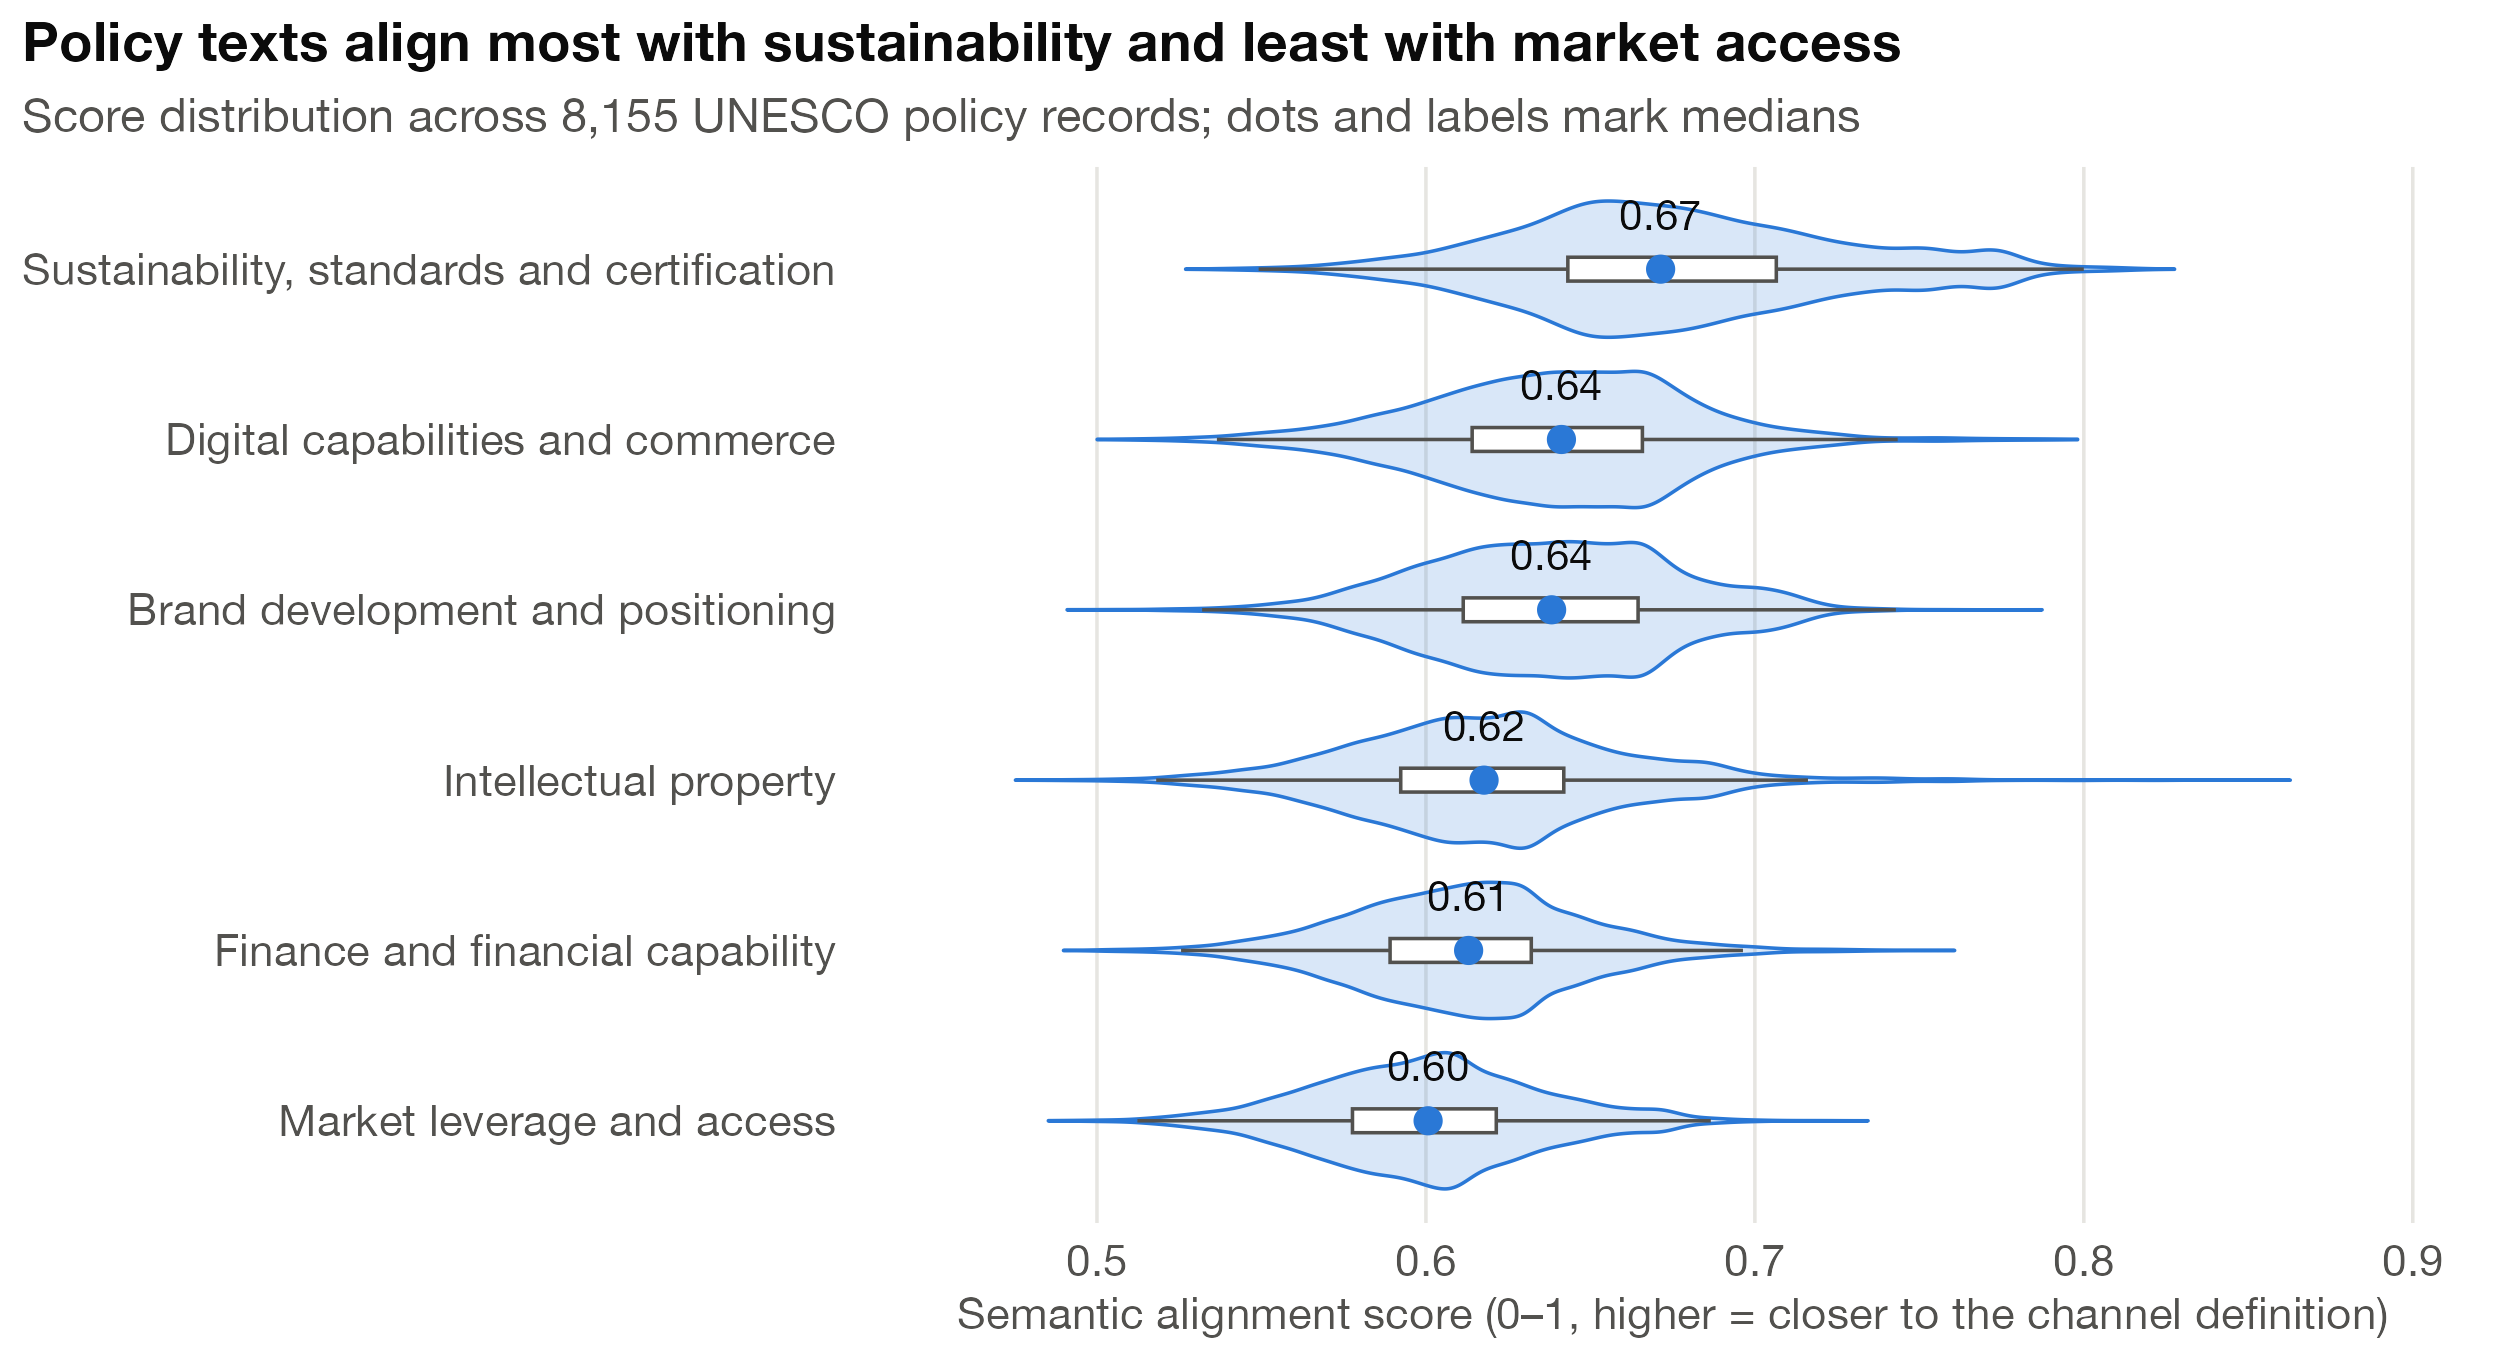
\includegraphics[width=\linewidth]{fig01_channel_attention.png}
  \figsource{Source: Author's calculations based on the UNESCO 2005 Convention policy monitoring platform.}
\end{figure}

\section{Coverage of the policy records}\label{sec:coverage}

Policy records are not evenly spread (Figure~\ref{fig:income}). High-income country-years average 24.0 records, middle-income 21.9 and low-income 17.2. This does not mean that richer countries have better policies. It reflects administrative capacity, reporting effort and the breadth of formal policy systems, and it is one reason the regressions control for GDP per capita.

\begin{figure}[H]
  \caption{UNESCO policy records by income group}\label{fig:income}
  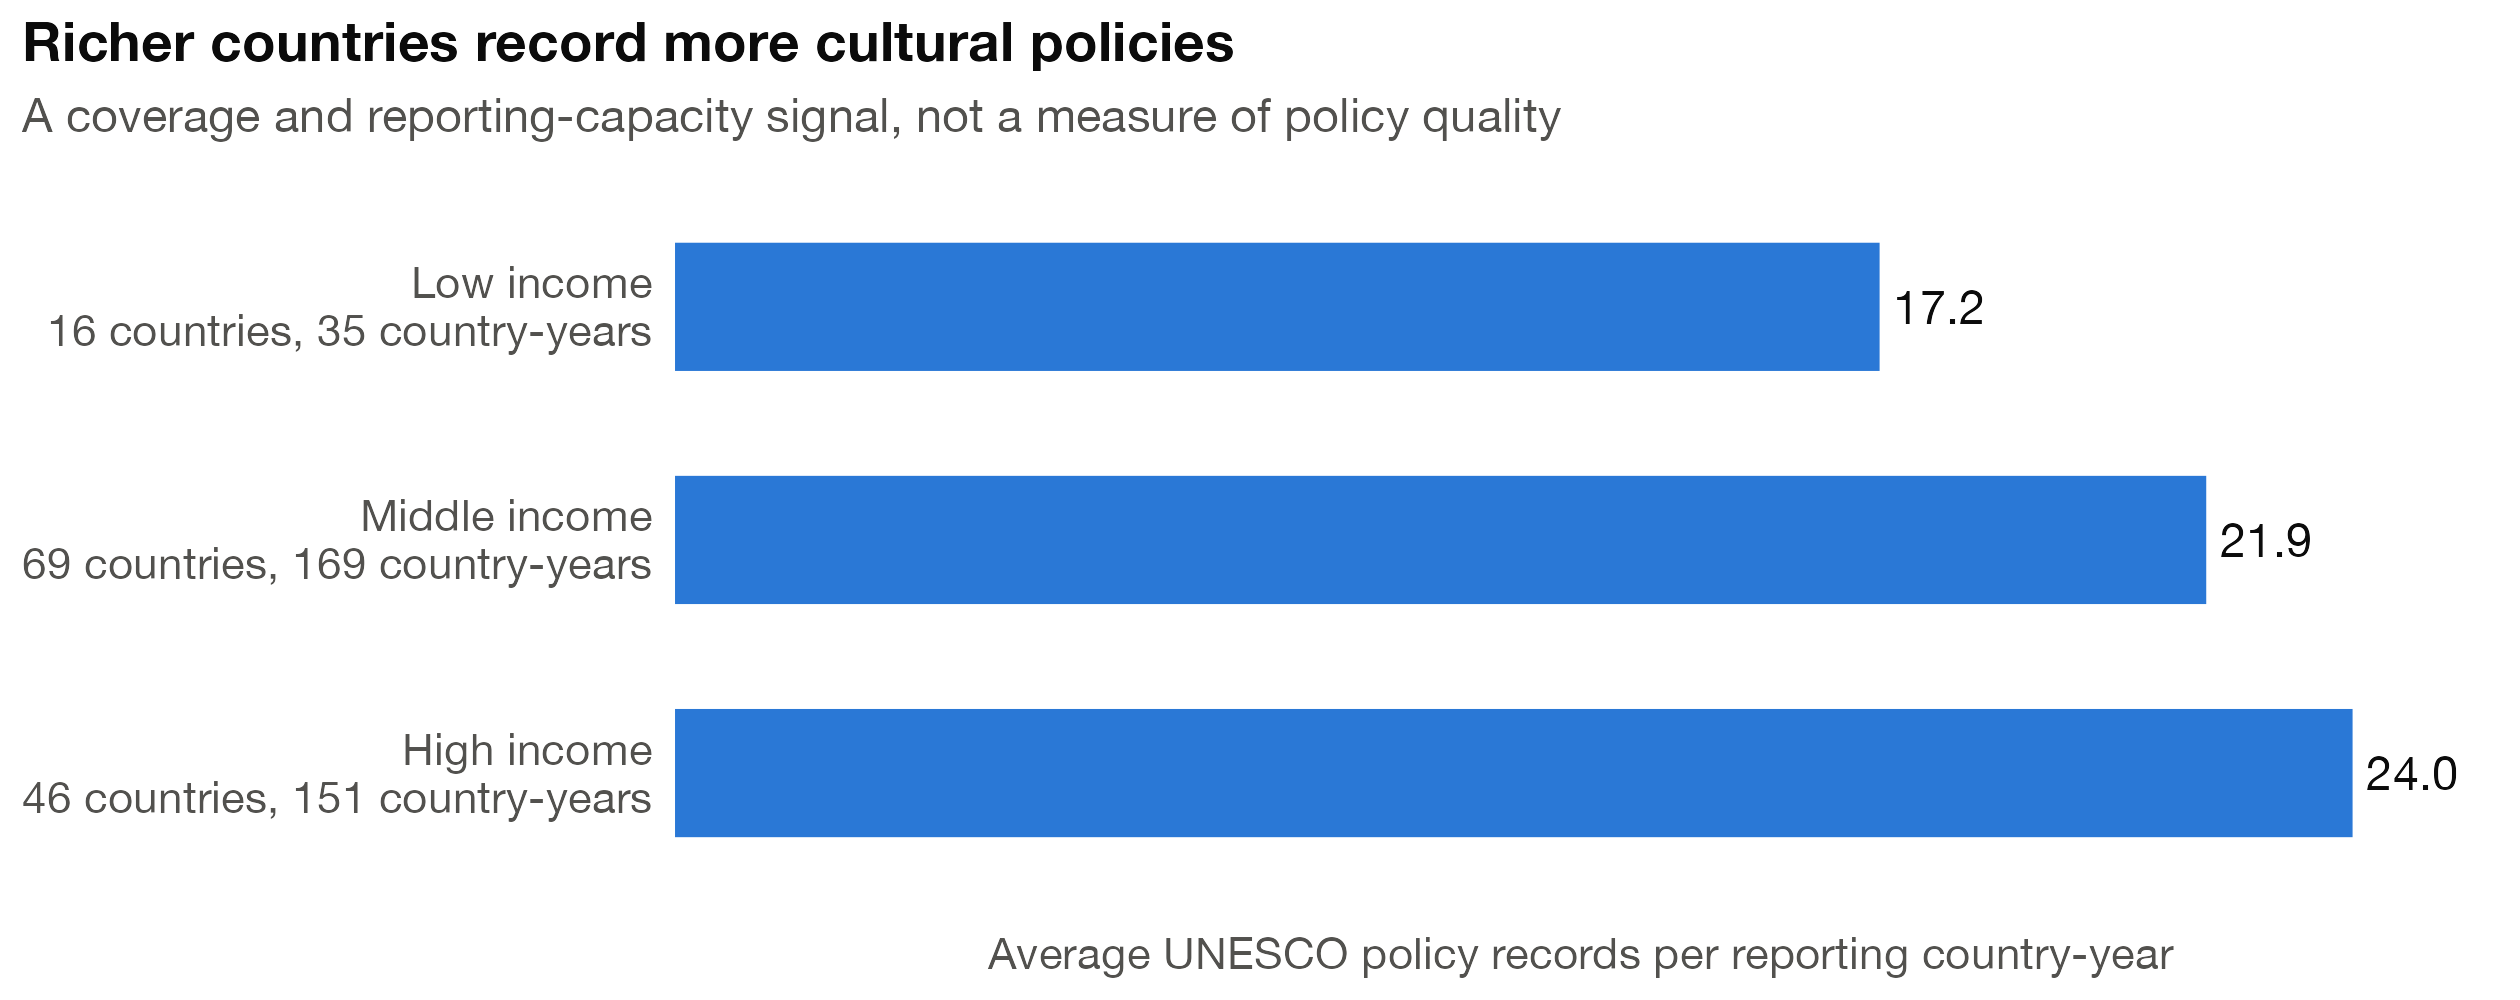
\includegraphics[width=\linewidth]{fig02_income_groups.png}
  \figsource{Source: Author's calculations based on UNESCO and World Bank FY2026 income groups.}
\end{figure}

Recorded volume has also grown (Figure~\ref{fig:volume}). The average per reporting country rose from 9 in 2012 to 32 in 2024. The quadrennial reporting years carry most countries, and the number of reporting countries more than doubled between the first and the last cycle, so part of the rise reflects who reports, not only how much. Firms surveyed from 2021 onwards are therefore matched to a richer and more recent record.

\begin{figure}[H]
  \caption{Recorded policy volume over time}\label{fig:volume}
  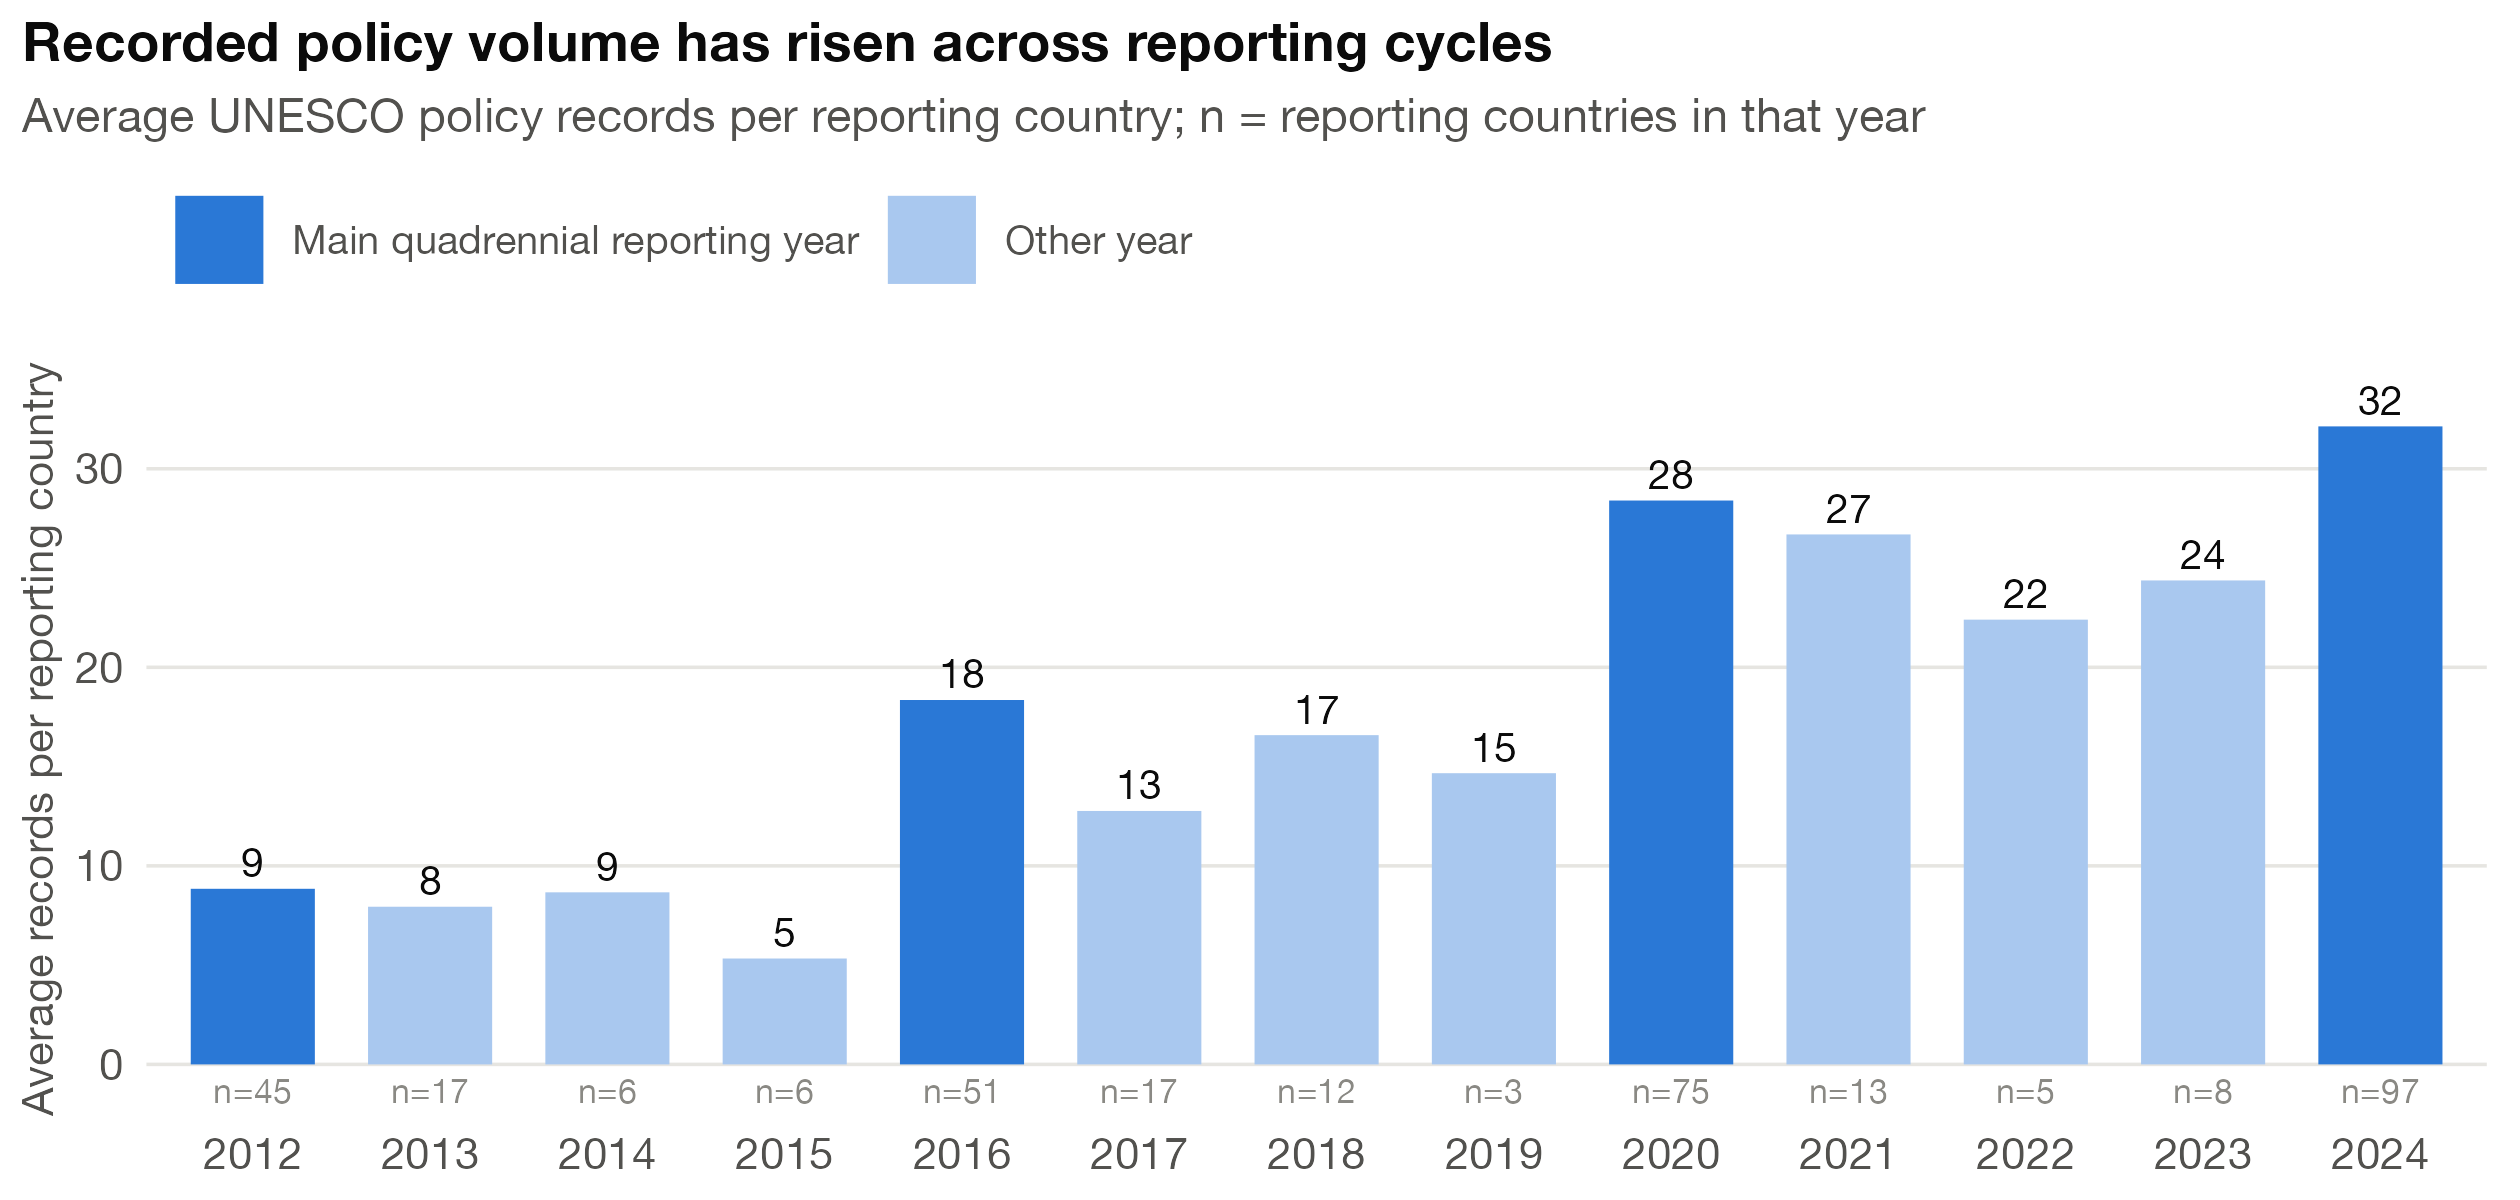
\includegraphics[width=\linewidth]{fig03_policy_volume.png}
  \figsource{Source: Author's calculations based on the UNESCO 2005 Convention policy monitoring platform.}
\end{figure}

\section{Empirical strategy}\label{sec:strategy}

The paper compares creative firms in high- and low-exposure country-waves in two ways. The first is a plain comparison of survey-weighted means, as used in the report's figures. The second is a regression that holds firm and country characteristics fixed, which is the evidence behind the report's technical appendix. All estimates come from a single Stata do-file that reads the raw WBES microdata, the creative-industry code list, the World Development Indicators and the policy scores.

For outcome $Y$ of firm $i$ in country $c$ surveyed in year $t$, and policy channel $k$, the estimated model is
\begin{equation*}
  Y_{ict} = \beta_k\, D^{(k)}_{ct} + \mathbf{X}_{ict}'\gamma + \mathbf{Z}_{c}'\delta + \lambda_t + \mu_{s(i)} + \eta_{\ell(i)} + \rho_{r(c)} + \varepsilon_{ict},
\end{equation*}
where $D^{(k)}_{ct}$ equals 1 if the country-wave's mean score for channel $k$ is above the median across country-waves (for overall policy volume, the number of recorded policies). $\mathbf{X}_{ict}$ contains log firm age, log employment (winsorized at the 1st and 99th percentiles) and female ownership, with missing values set to the median and a missingness indicator included. $\mathbf{Z}_{c}$ contains log GDP per capita, log population and access to electricity. $\lambda_t$, $\mu_{s}$, $\eta_{\ell}$ and $\rho_{r}$ are survey-year, ISIC division, legal-status and World Bank region fixed effects. Models are estimated by weighted least squares with the country-normalized weights; binary outcomes are linear probability models. Standard errors are clustered by country, the level at which exposure is assigned.

\section{Creative firms and policy exposure}\label{sec:desc}

Each figure in this section has two parts. The bars, as prepared for the report, compare the survey-weighted share (or average) of an outcome among creative firms in country-waves below and above the median exposure for the relevant channel; they control for nothing. Beneath each pair of bars is the corresponding regression estimate: the adjusted difference between above- and below-median country-waves, with a 90\% confidence interval, after controlling for firm age, size and female ownership, GDP per capita, population and electricity access, and survey-year, industry, legal-status and region fixed effects, with standard errors clustered by country. These estimates are the background evidence for the report's technical appendix. Stars mark $p<0.10$ ($^{*}$), $p<0.05$ ($^{**}$) and $p<0.01$ ($^{***}$); Table~\ref{tab:reg} in Section~\ref{sec:reg} reports standard errors and sample sizes.

\subsection{Overall policy volume}

\begin{figure}[H]
  \caption{Overall policy count: creative firms in high-policy-count countries innovate and export more}
  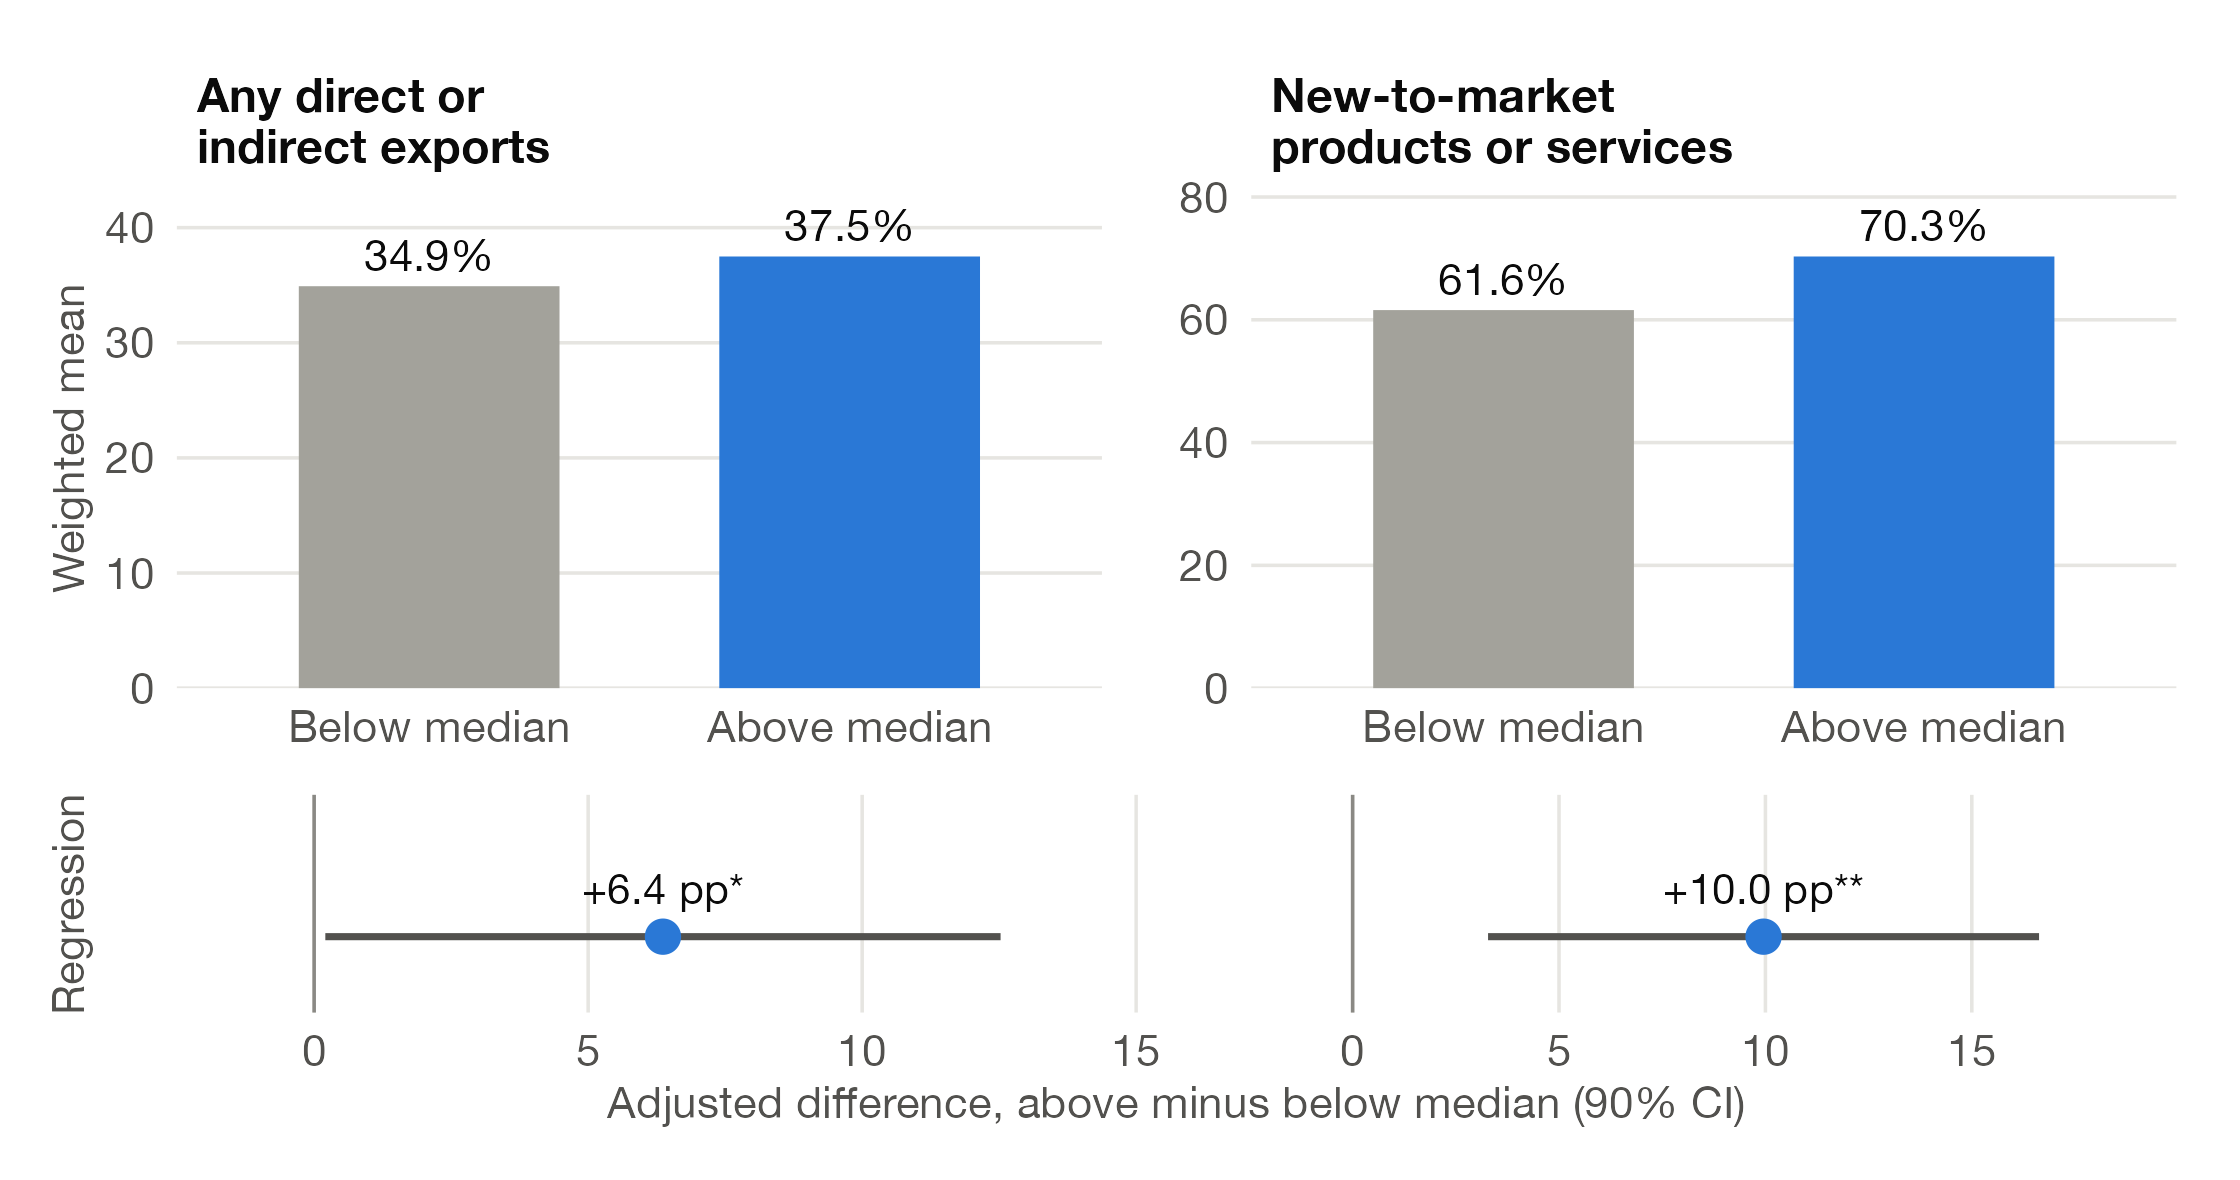
\includegraphics[width=0.85\linewidth]{fig04_overall_policy_count.png}
  \figsource{Note: Bars show survey-weighted means for creative firms in country-waves below (grey) and above (blue) the median exposure, as prepared for the report. Below each pair, the regression estimate of the adjusted difference with its 90\% confidence interval (background evidence for the report's technical appendix). Source: Author's calculations based on UNESCO and WBES.}
\end{figure}

Creative firms in countries that record more policies are more likely to bring products or services new to their market: 70.3\% against 61.6\%, and $+$10.0 percentage points after controls ($p=0.017$). Exporting is somewhat more common (37.5\% against 34.9\%; $+$6.4 points, $p=0.094$), but the evidence is weaker.

\subsection{Intellectual property}

\begin{figure}[H]
  \caption{Intellectual property: where policy stresses IP, creative firms upgrade processes and reward output}
  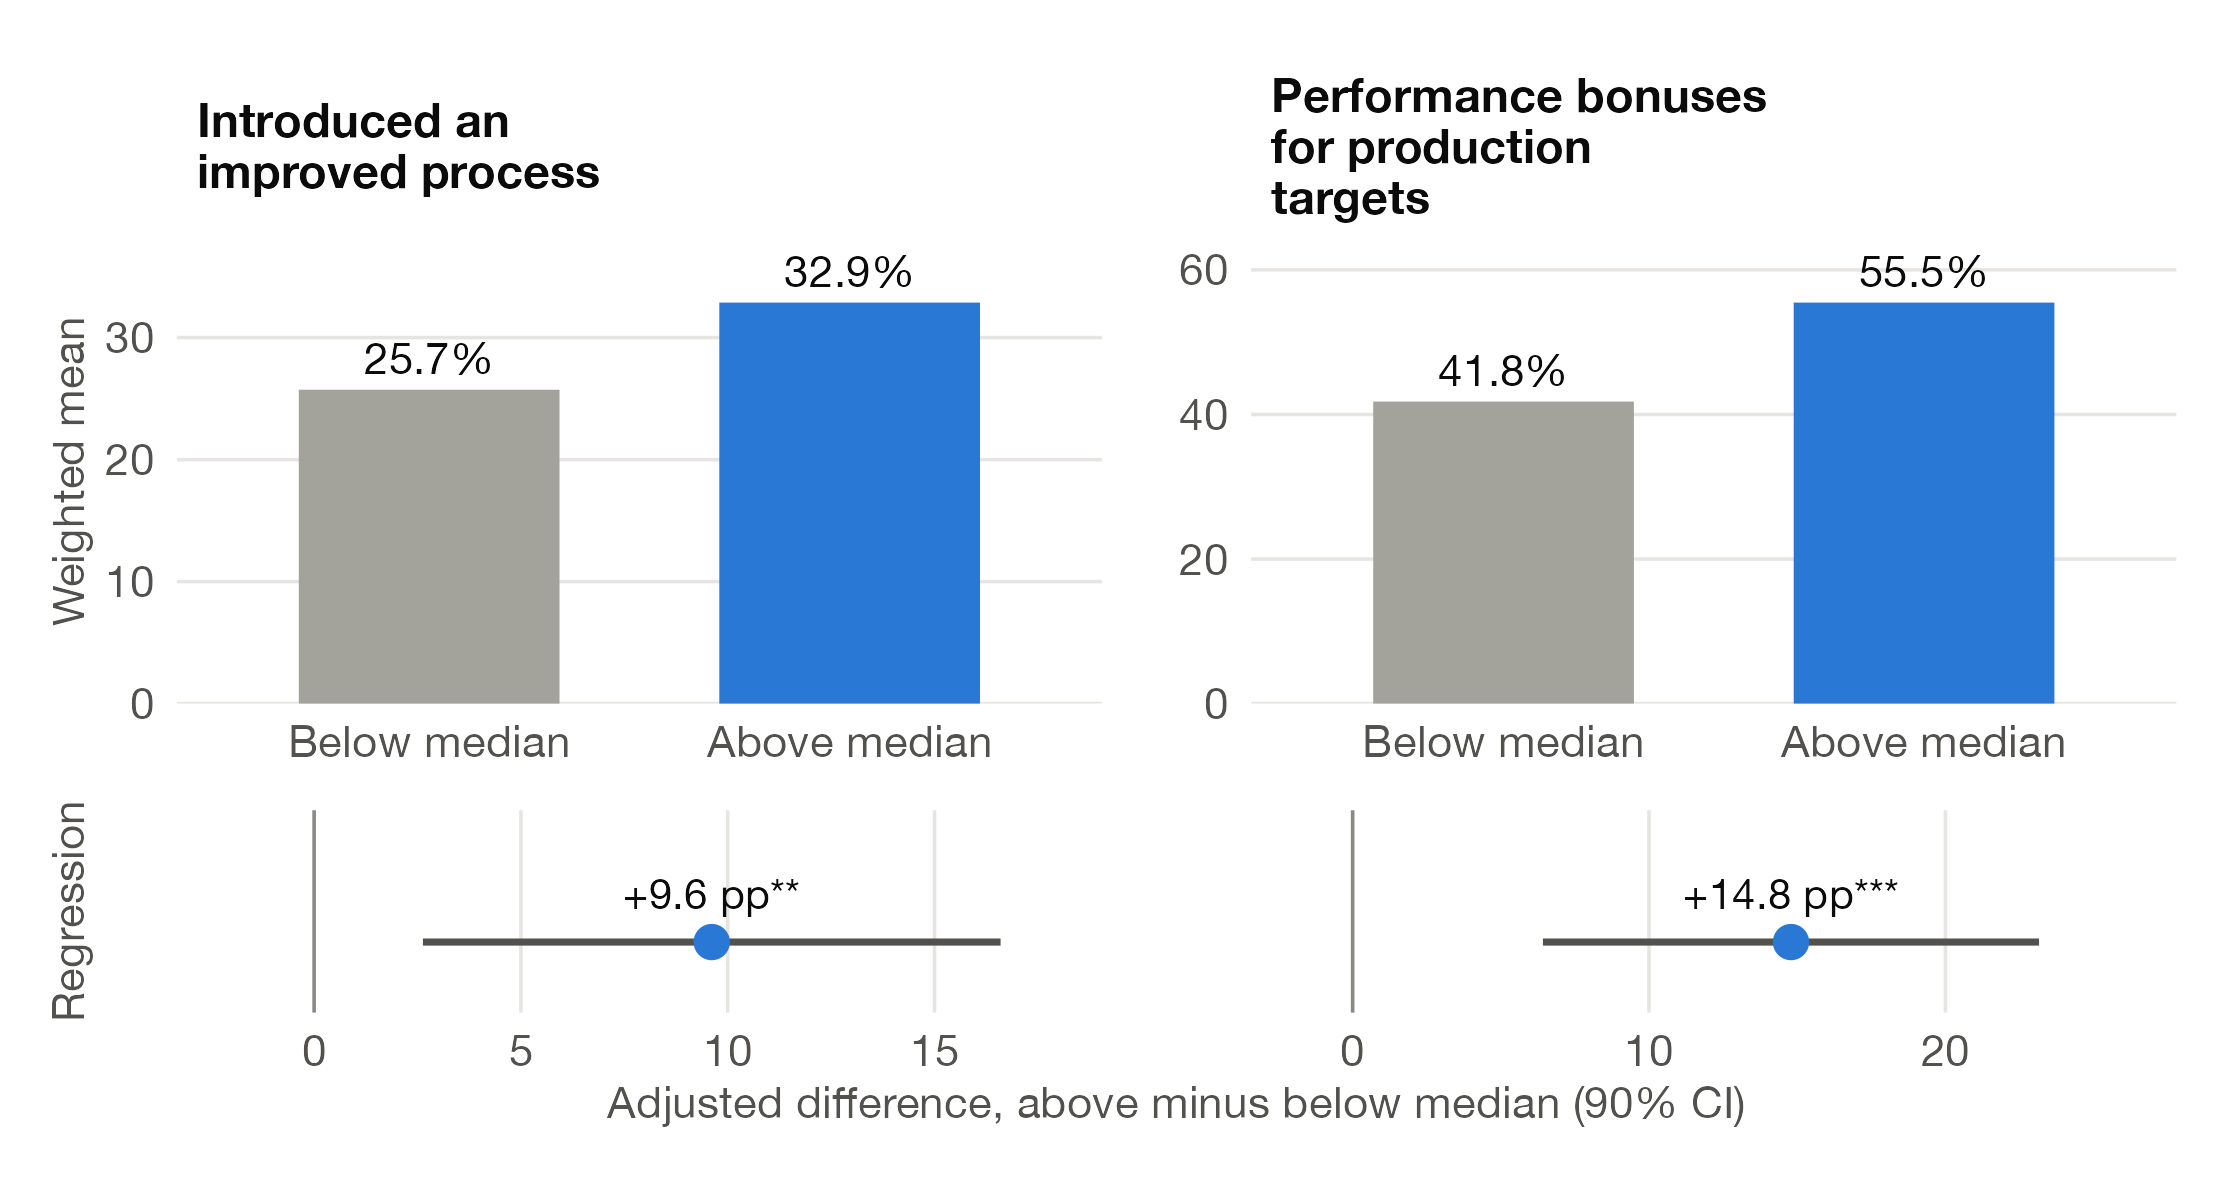
\includegraphics[width=0.85\linewidth]{fig05_intellectual_property.png}
  \figsource{Note: As in Figure 4. Source: Author's calculations based on UNESCO and WBES.}
\end{figure}

Where policy texts focus more on intellectual property, creative firms are more likely to have introduced an improved process (32.9\% against 25.7\%; $+$9.6 points after controls, $p=0.027$) and to pay performance bonuses tied to production targets (55.5\% against 41.8\%; $+$14.8 points, $p=0.005$). Both point to firms that invest in and reward know-how, the base on which intellectual property is built.

\subsection{Brand development and positioning}

\begin{figure}[H]
  \caption{Brand development and positioning: where policy stresses branding, creative firms report more pricing power}
  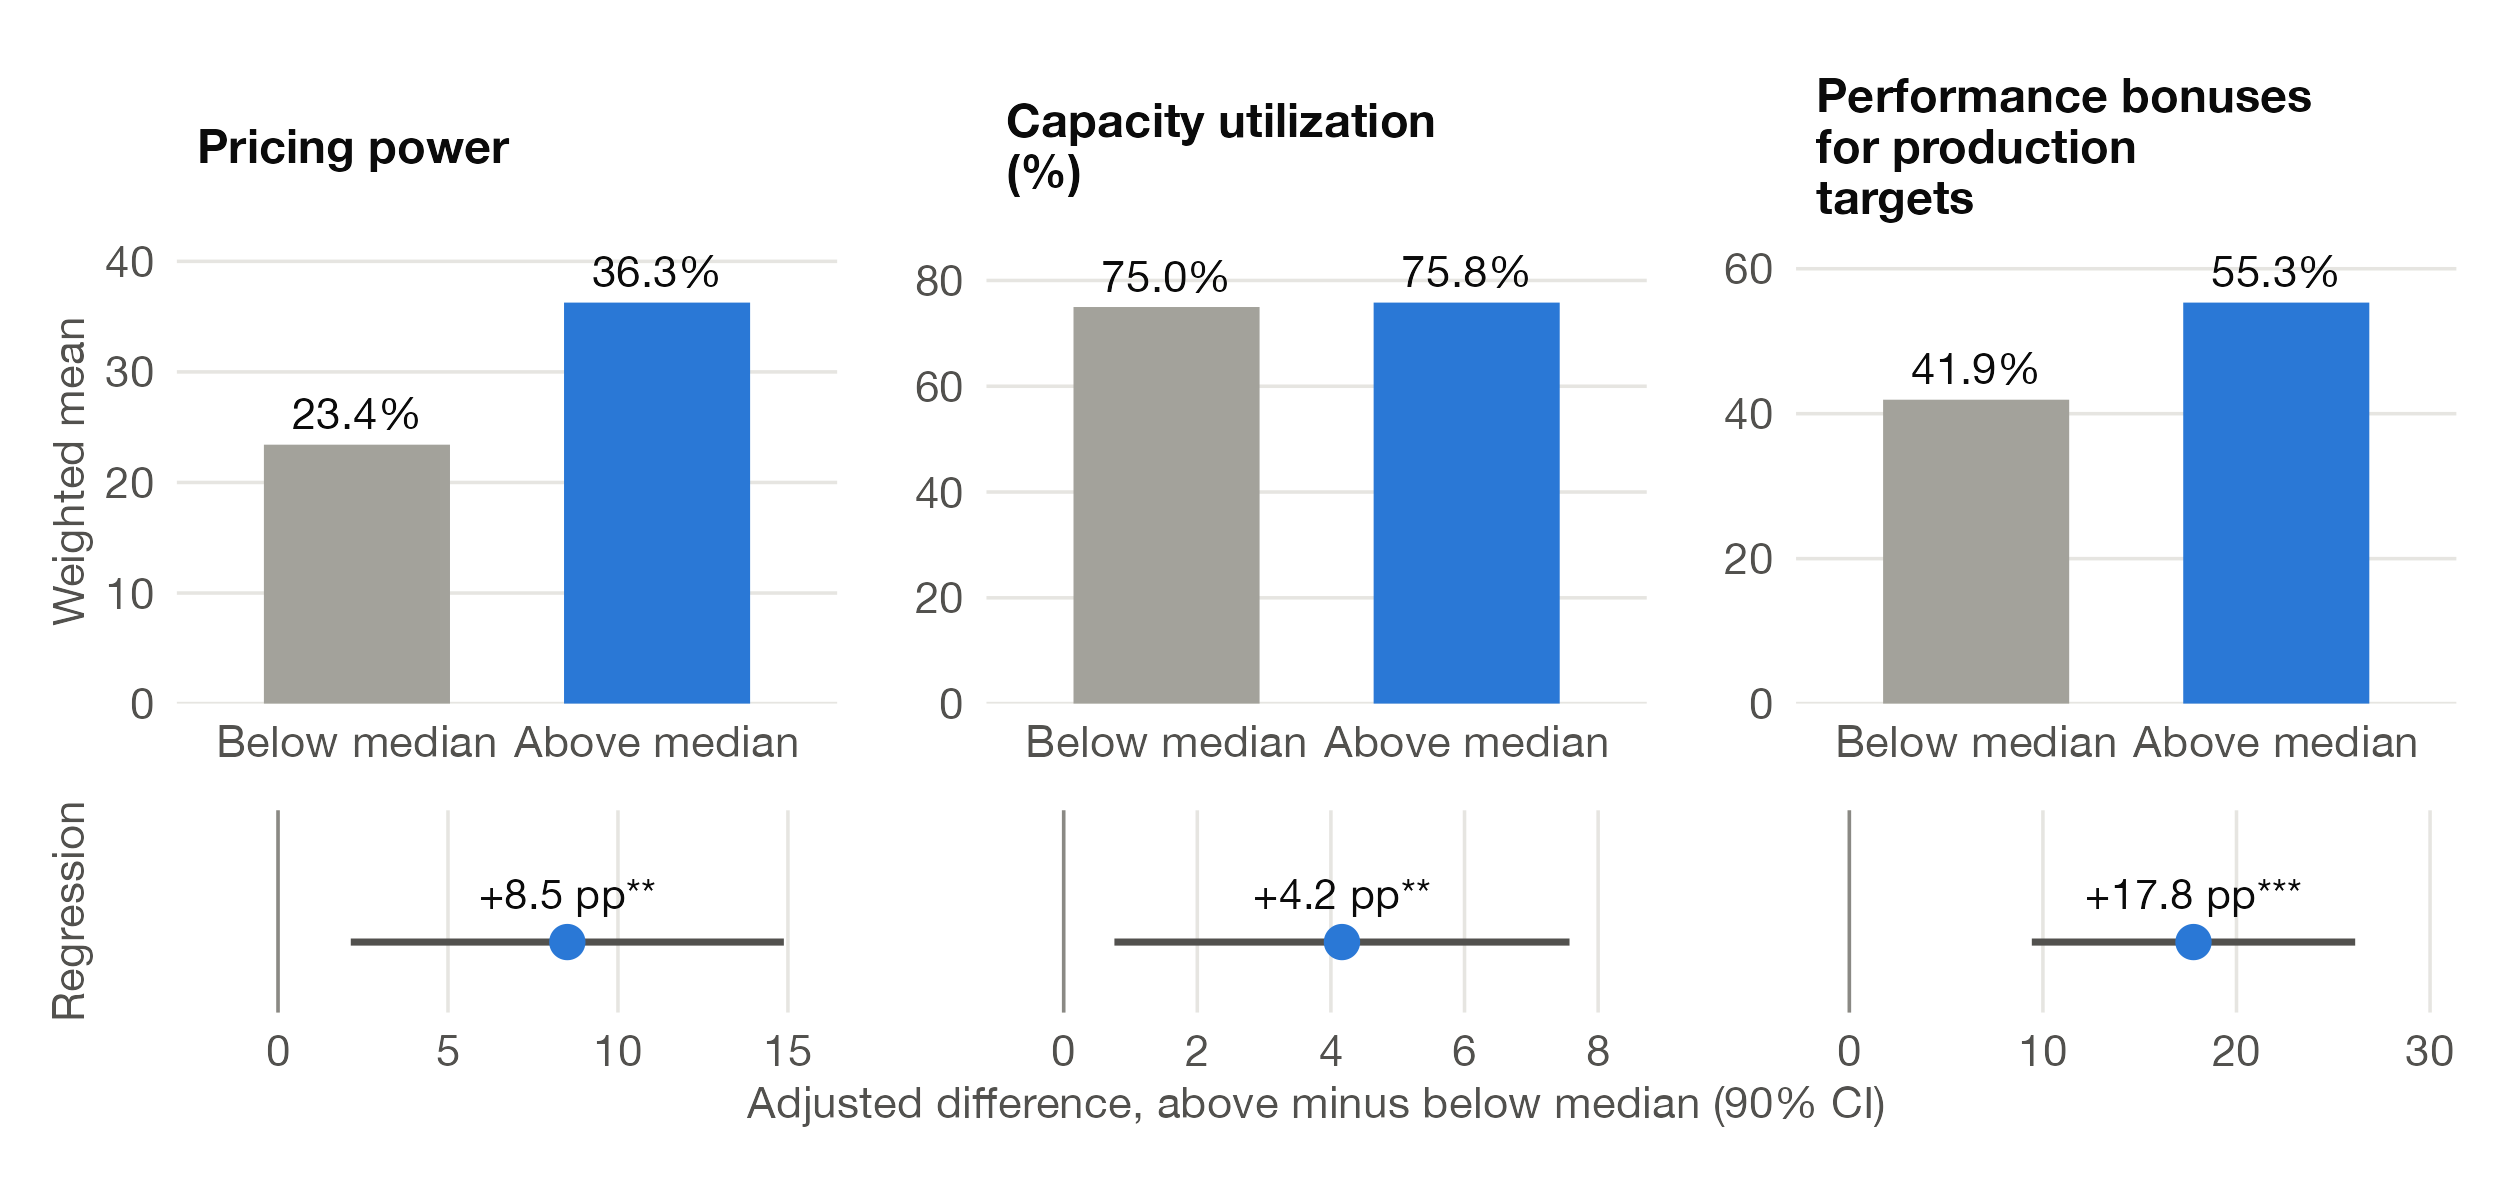
\includegraphics[width=0.95\linewidth]{fig06_brand_development_and_positioning.png}
  \figsource{Note: As in Figure 4. Source: Author's calculations based on UNESCO and WBES.}
\end{figure}

Pricing power, the clearest observable sign of a brand that customers value, is reported by 36.3\% of creative firms in high-branding countries against 23.4\% elsewhere ($+$8.5 points after controls, $p=0.031$). Performance bonuses are again more common ($+$17.8 points, $p<0.001$). Capacity utilization is similar in raw terms (75.8\% against 75.0\%) but higher once firm and country differences are accounted for ($+$4.2 points, $p=0.048$).

\subsection{Market leverage and access}

\begin{figure}[H]
  \caption{Market leverage and access: where policy stresses market access, imports clear faster}
  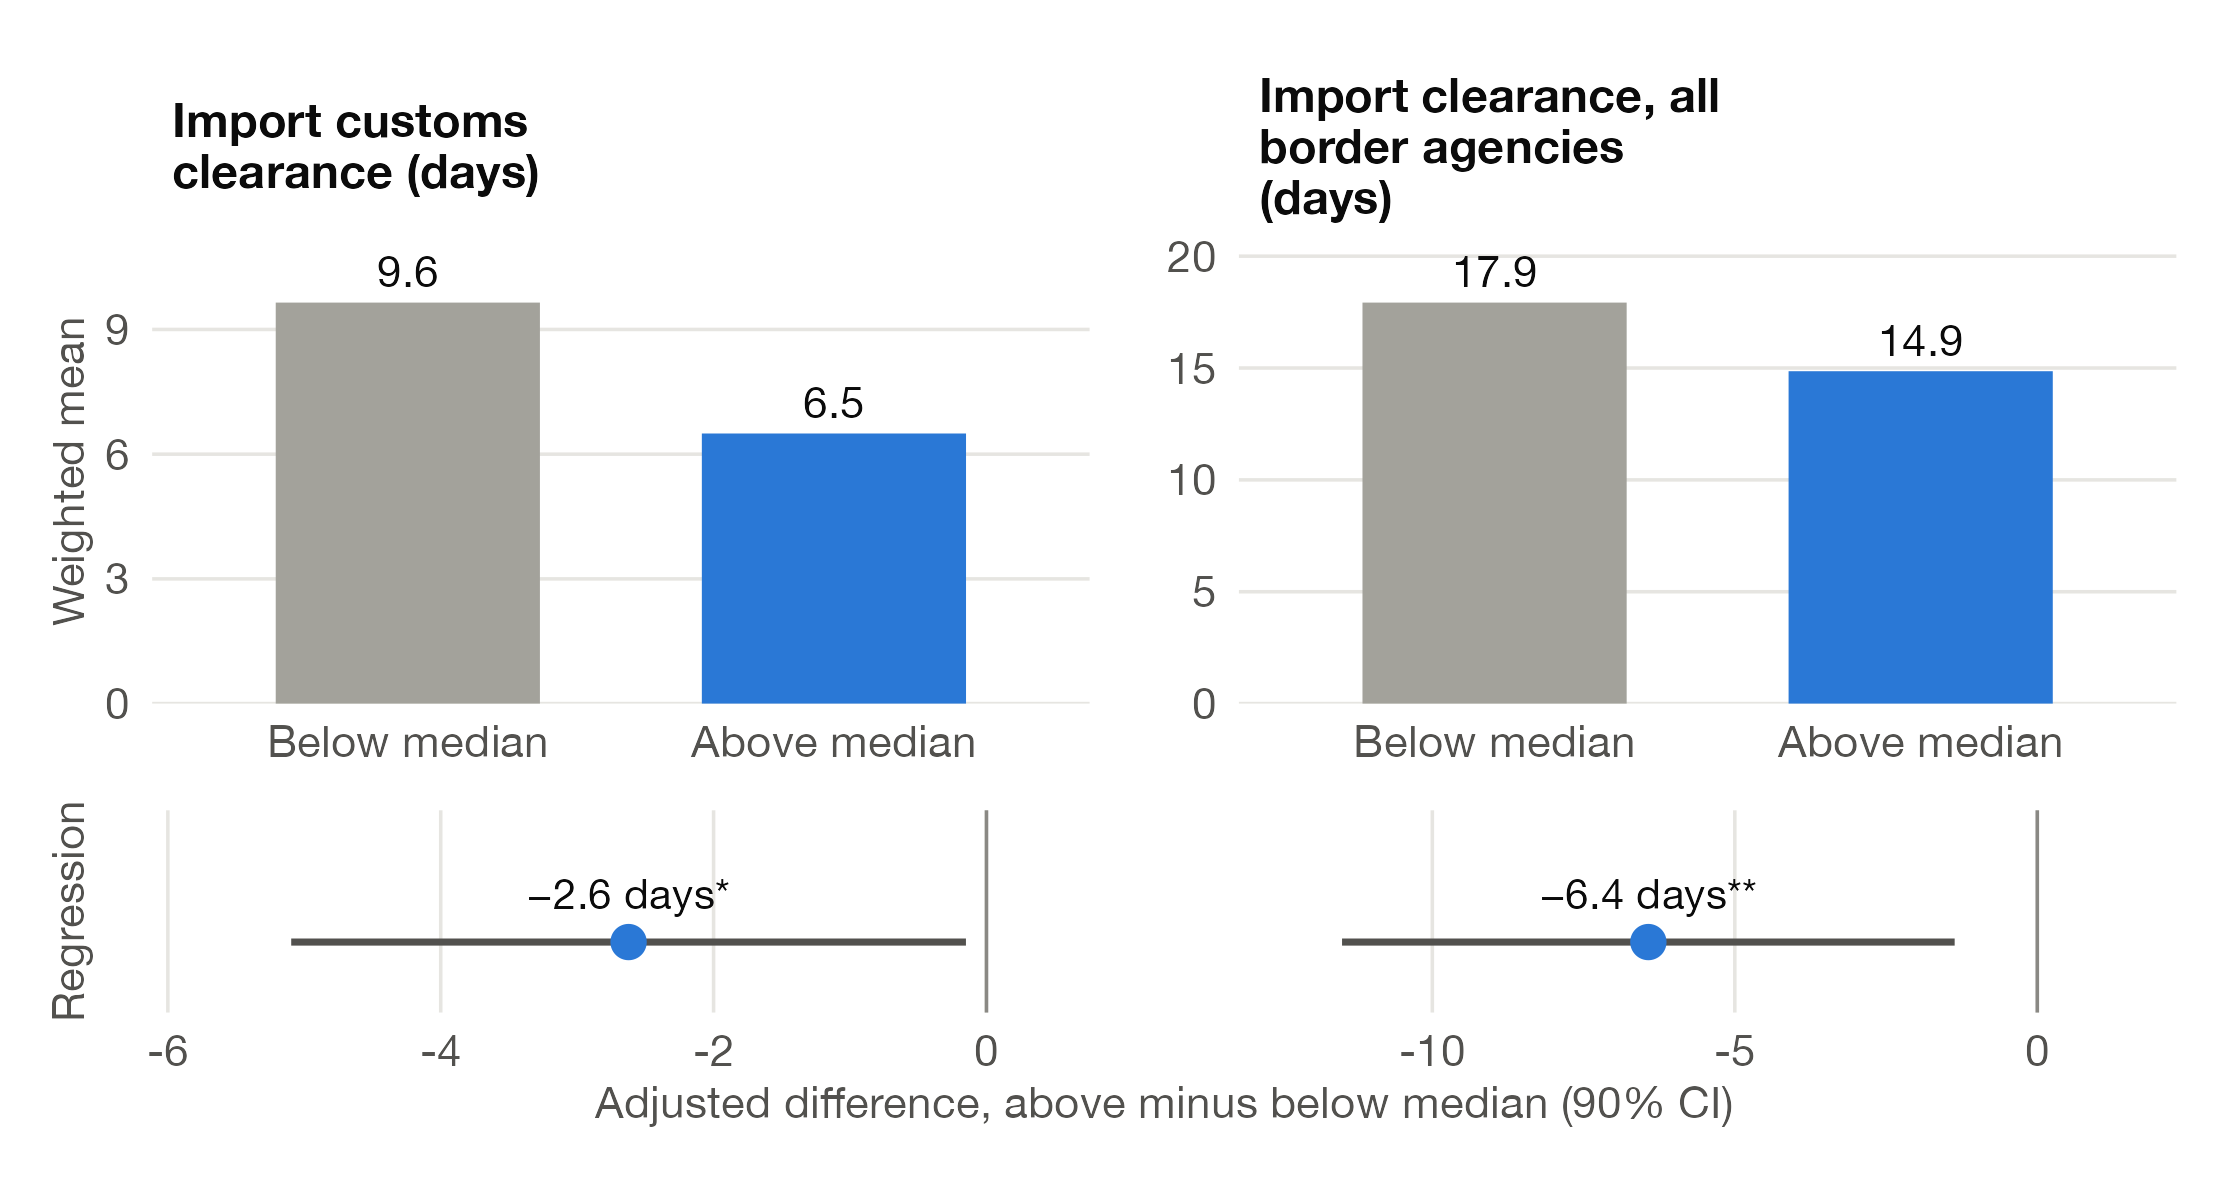
\includegraphics[width=0.85\linewidth]{fig07_market_leverage_and_access.png}
  \figsource{Note: As in Figure 4. Source: Author's calculations based on UNESCO and WBES.}
\end{figure}

Where policies focus more on market access, imported inputs clear the border faster: 14.9 days for all border agencies against 17.9 days ($-$6.4 days after controls, $p=0.042$), and 6.5 against 9.6 days for customs alone ($-$2.6 days, $p=0.086$). Fewer firms import directly, so these samples are smaller.

\subsection{Digital capabilities and commerce}

\begin{figure}[H]
  \caption{Digital capabilities and commerce: where policy stresses digital, e-payments arrive faster and training is wider}
  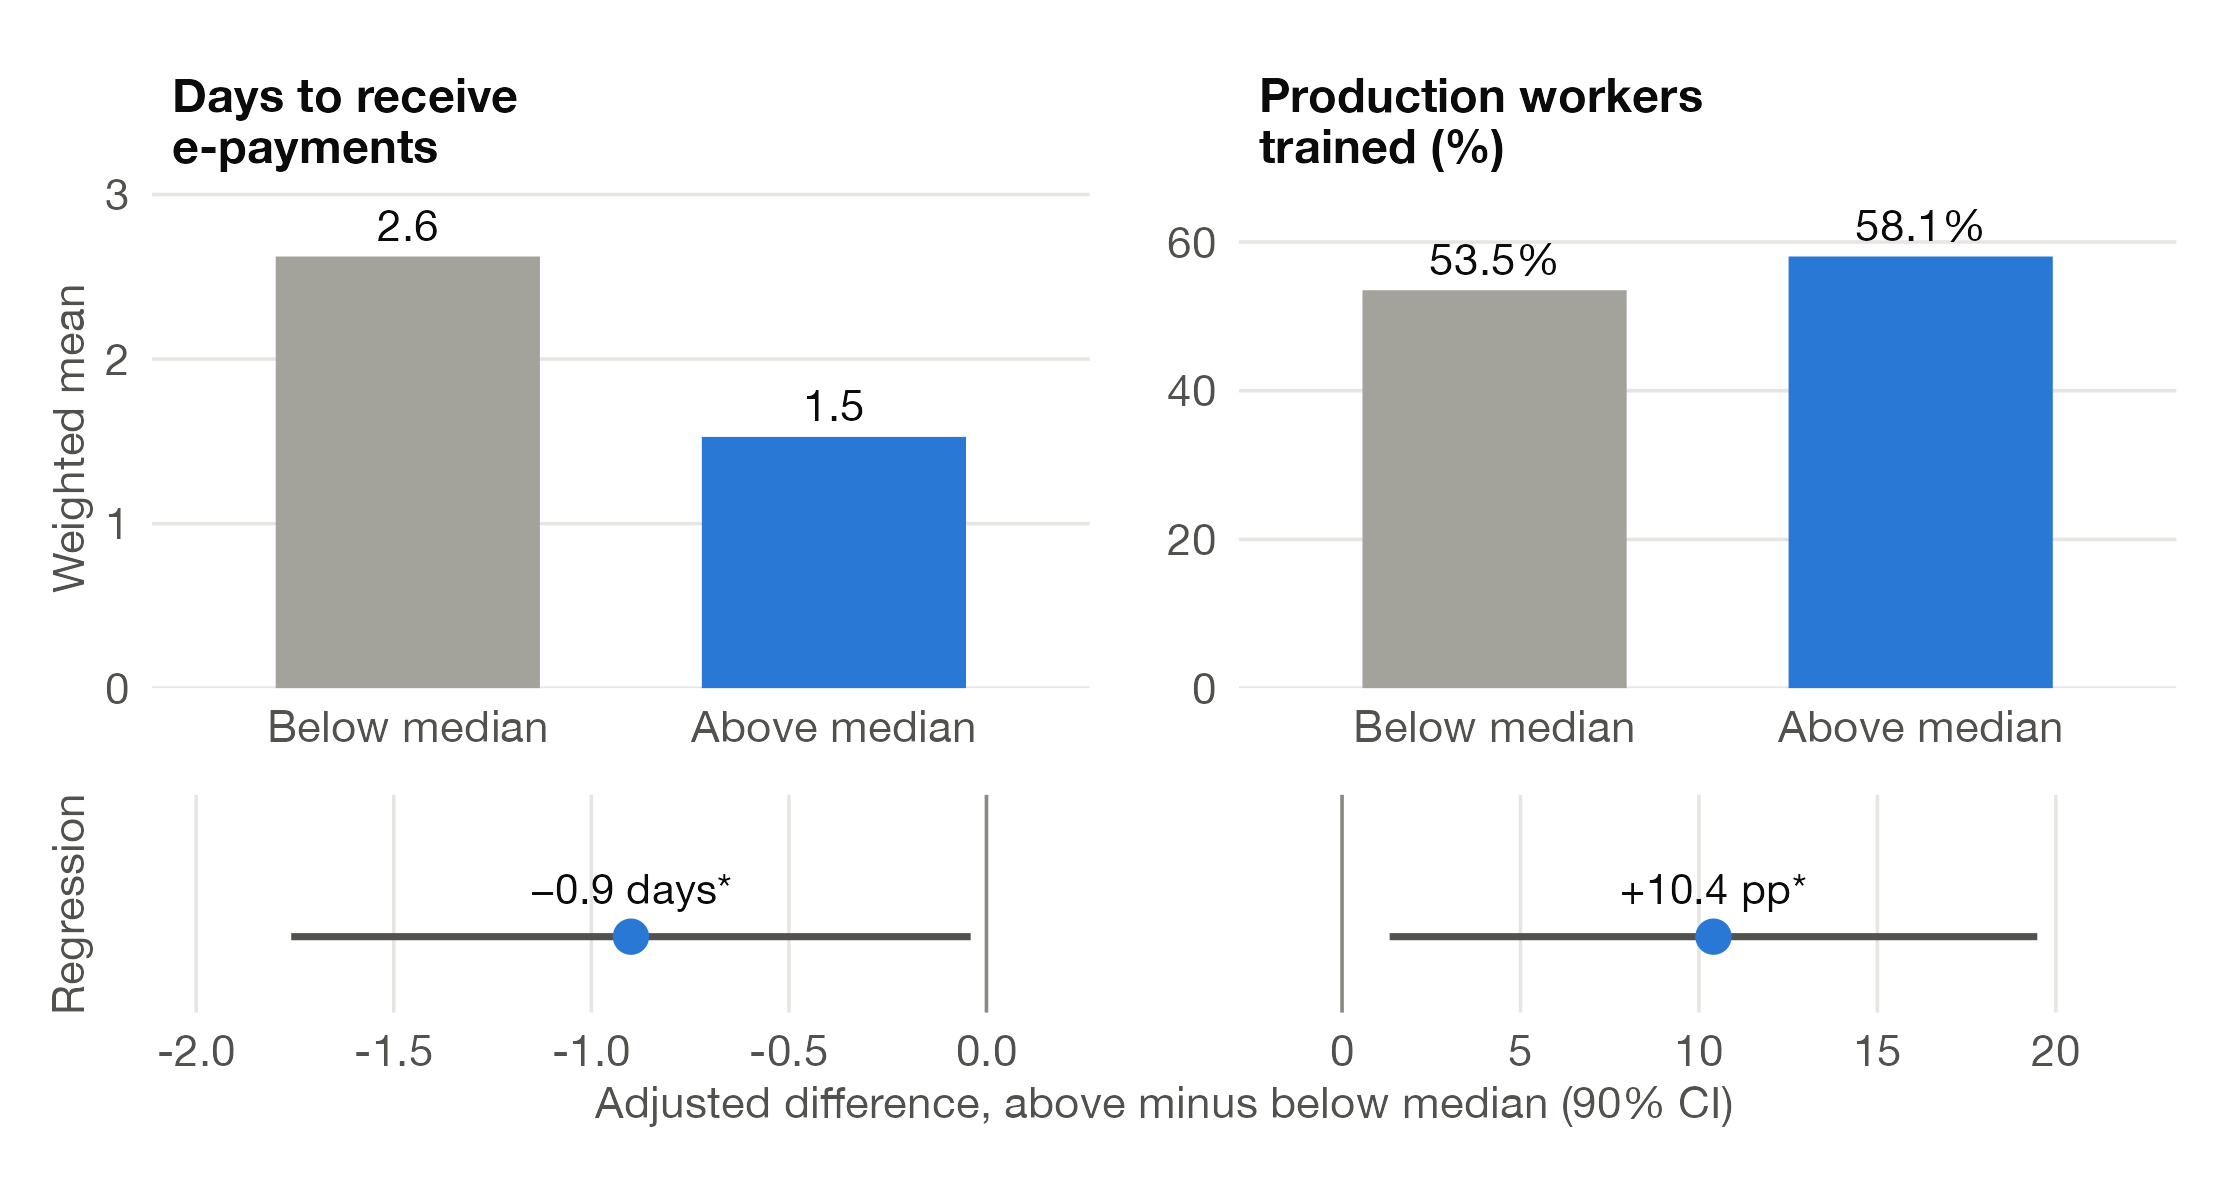
\includegraphics[width=0.85\linewidth]{fig08_digital_capabilities_and_commerce.png}
  \figsource{Note: As in Figure 4. Source: Author's calculations based on UNESCO and WBES.}
\end{figure}

In countries with a stronger digital focus, creative firms receive electronic payments faster (1.5 against 2.6 days; $-$0.9 days after controls, $p=0.090$) and train a larger share of their production workers (58.1\% against 53.5\%; $+$10.4 points, $p=0.063$). Both adjusted differences are marginal.

\subsection{Finance and financial capability}

\begin{figure}[H]
  \caption{Finance and financial capability: where policy stresses finance, creative firms face fewer finance obstacles}
  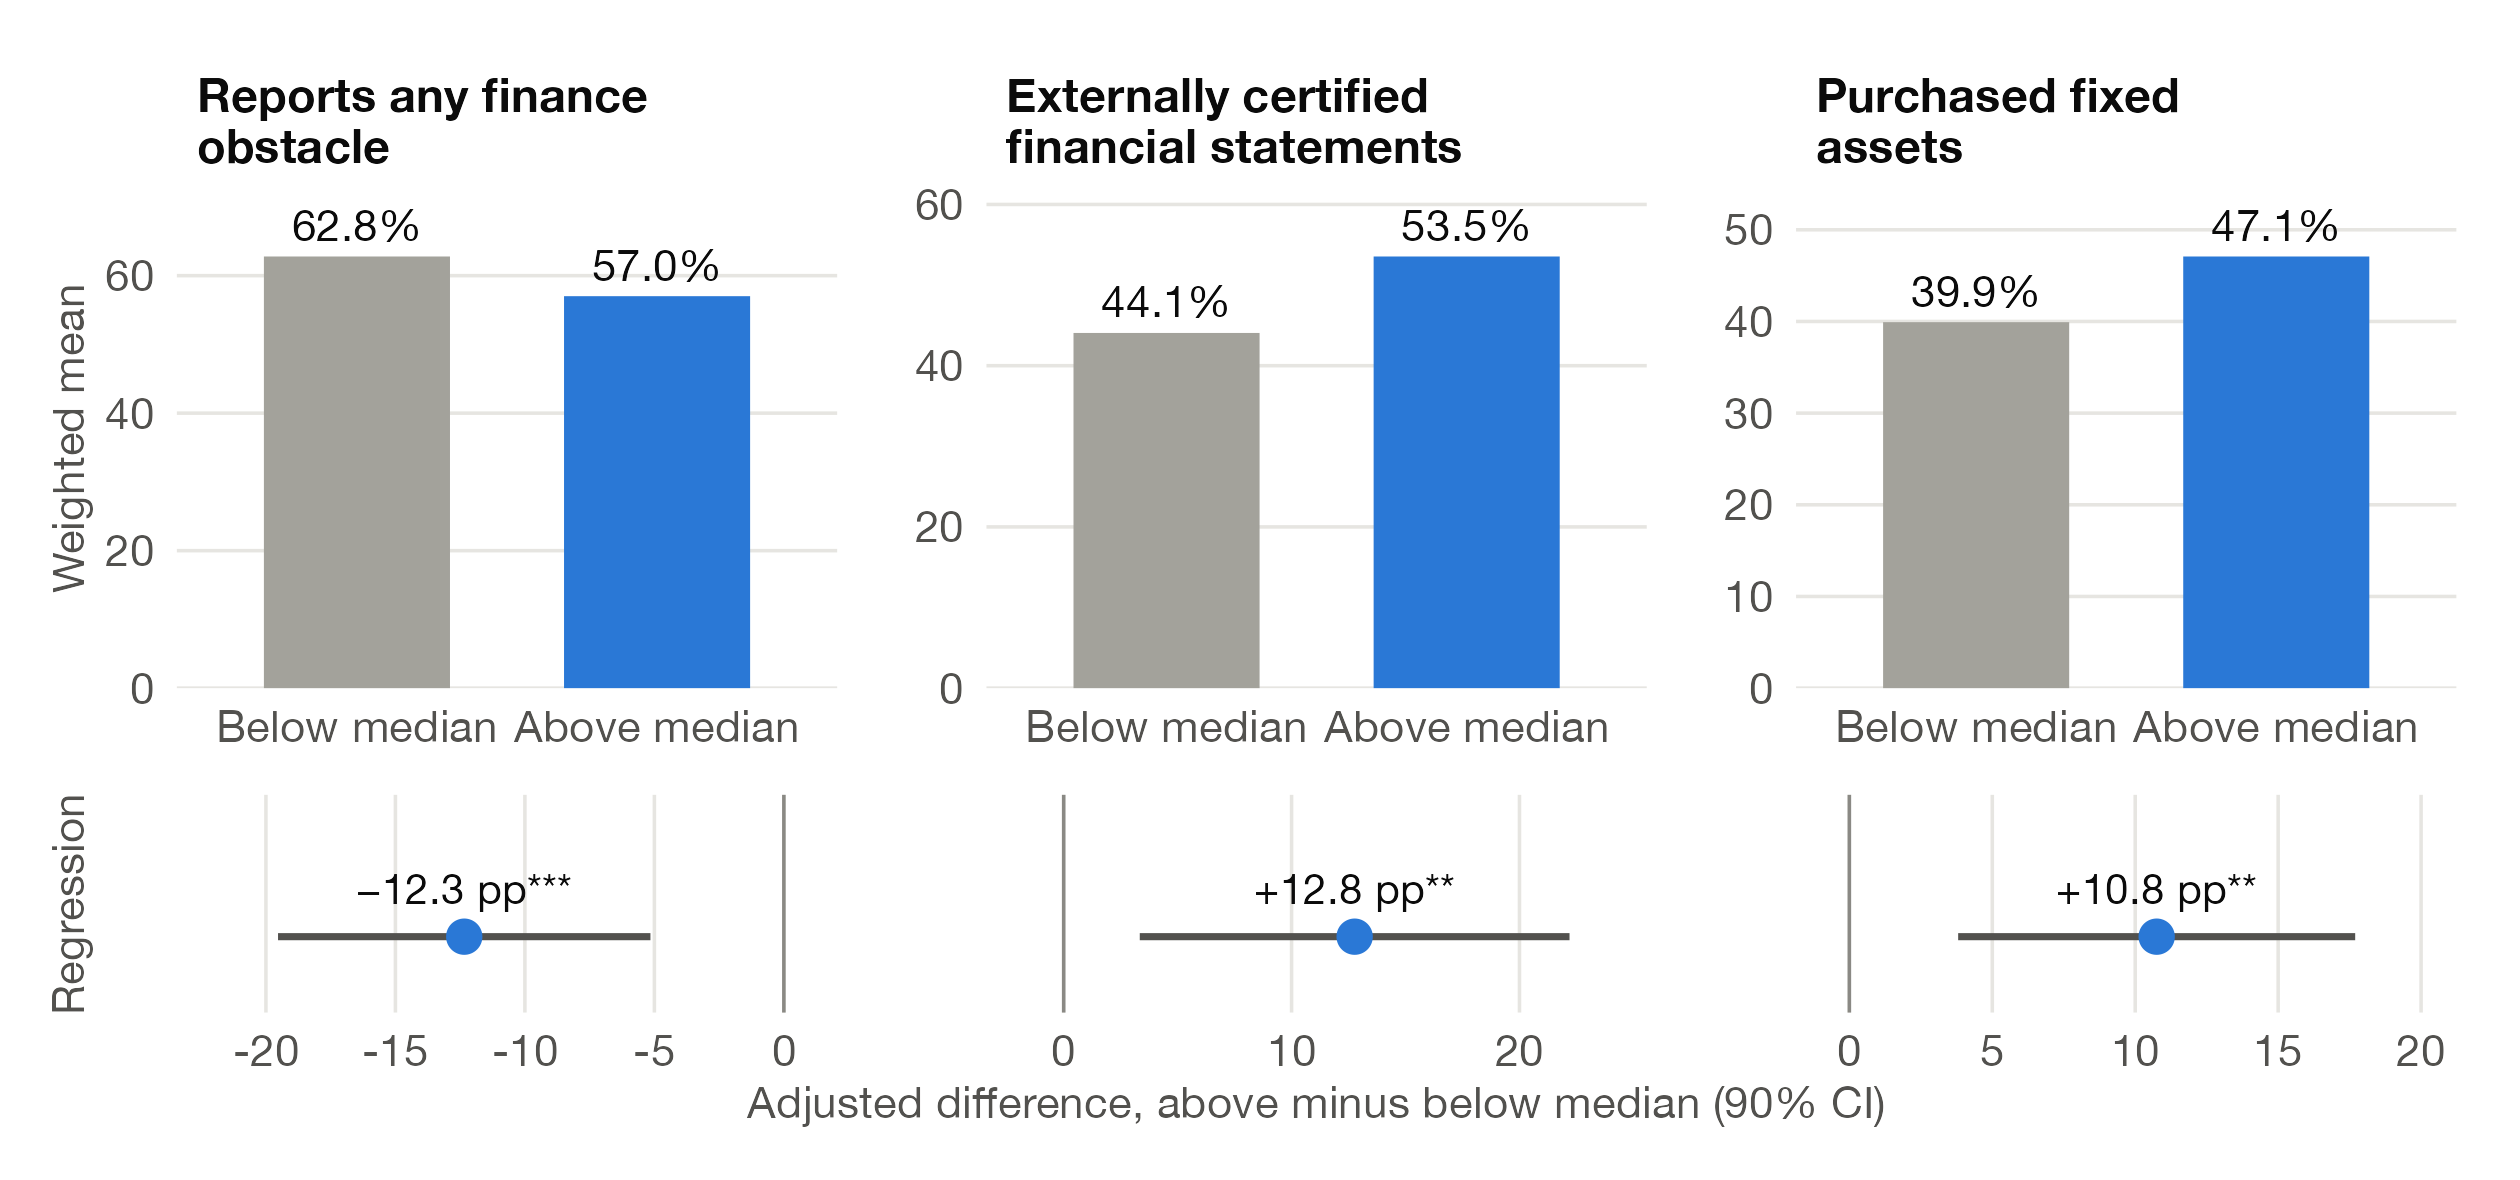
\includegraphics[width=0.95\linewidth]{fig09_finance_and_financial_capability.png}
  \figsource{Note: As in Figure 4. Source: Author's calculations based on UNESCO and WBES.}
\end{figure}

Finance shows the clearest pattern. In countries with more finance-focused policies, fewer creative firms report finance as an obstacle (57.0\% against 62.8\%; $-$12.3 points after controls, $p=0.006$), more have bought fixed assets (47.1\% against 39.9\%; $+$10.8 points, $p=0.013$), and more have externally certified financial statements (53.5\% against 44.1\%; $+$12.8 points, $p=0.029$), which lenders often require.

\subsection{Sustainability, standards and certification}

\begin{figure}[H]
  \caption{Sustainability, standards and certification: where policy stresses sustainability, more creative firms use solar and upgrade processes}
  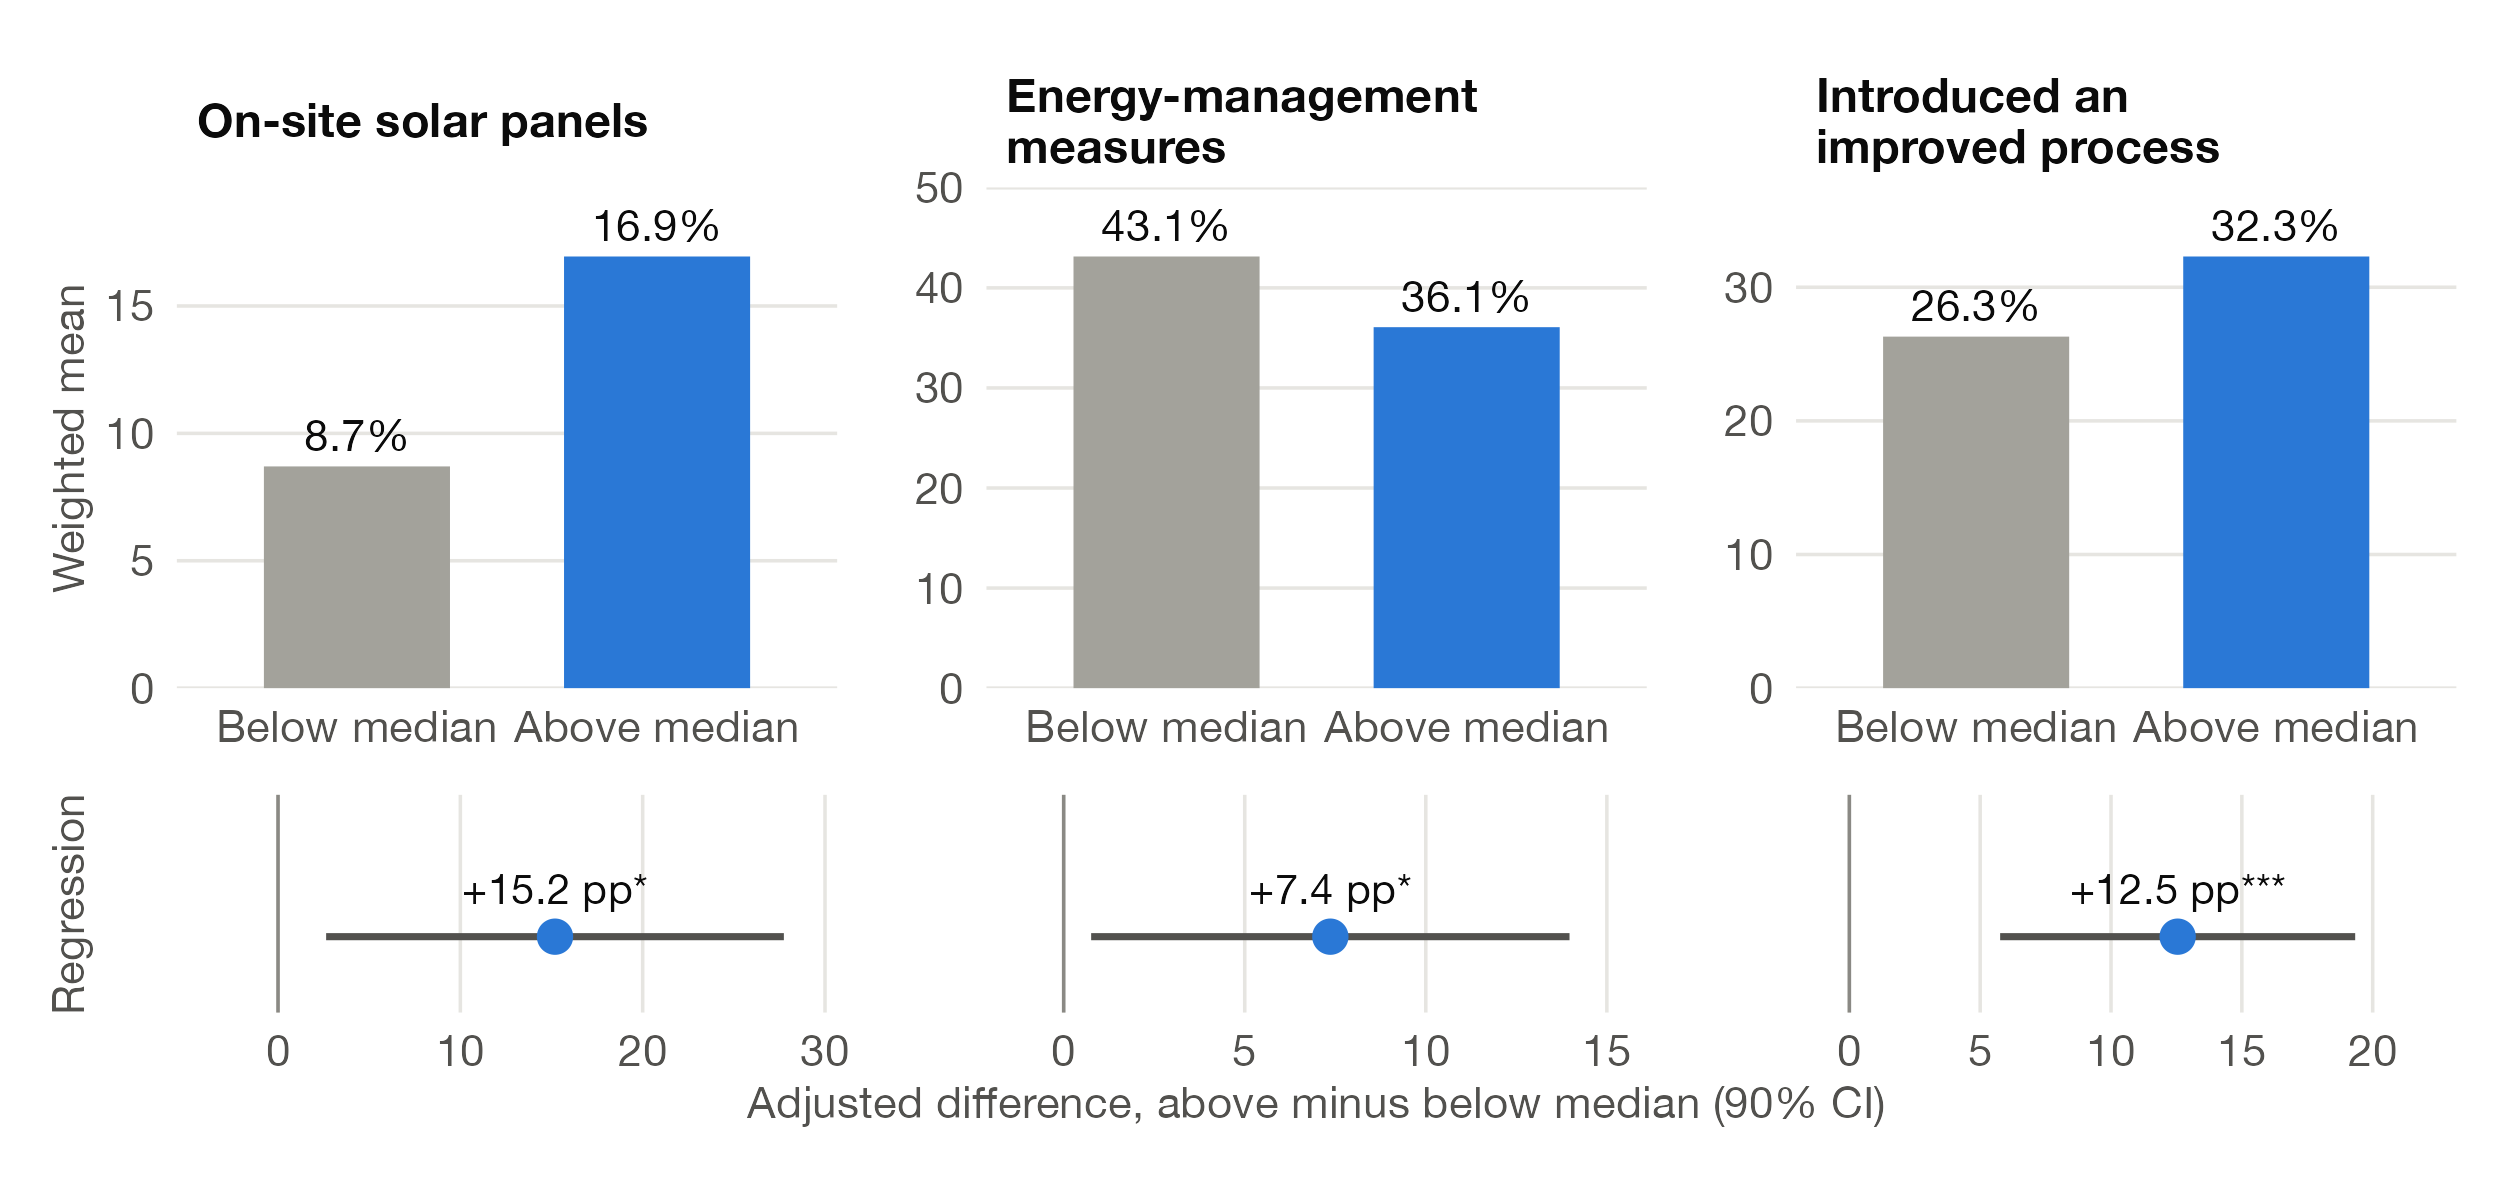
\includegraphics[width=0.95\linewidth]{fig10_sustainability.png}
  \figsource{Note: As in Figure 4. Source: Author's calculations based on UNESCO and WBES.}
\end{figure}

On-site solar panels are used by 16.9\% of creative firms in high-sustainability countries against 8.7\% elsewhere ($+$15.2 points, $p=0.061$; only 20 countries ask this question). Process upgrading is more common ($+$12.5 points, $p=0.003$). Energy-management measures run the other way in raw terms (36.1\% against 43.1\%) but turn positive after controls ($+$7.4 points, $p=0.071$), so this result should be read with care.

\section{Regression results}\label{sec:reg}

Figure~\ref{fig:allcoef} brings the 17 estimates from Section~\ref{sec:desc} together and places them on a common scale by dividing each coefficient by the outcome's weighted standard deviation. Table~\ref{tab:reg} reports them in original units, with standard errors and sample sizes. Eleven of the 17 estimates are significant at the 5\% level and all 17 at the 10\% level, which partly reflects how the outcomes were selected (Section~\ref{sec:disc}). Most associations are between 0.15 and 0.35 standard deviations; the largest are for on-site solar panels and performance bonuses.

\begin{figure}[H]
  \caption{Standardized adjusted associations, all channels}\label{fig:allcoef}
  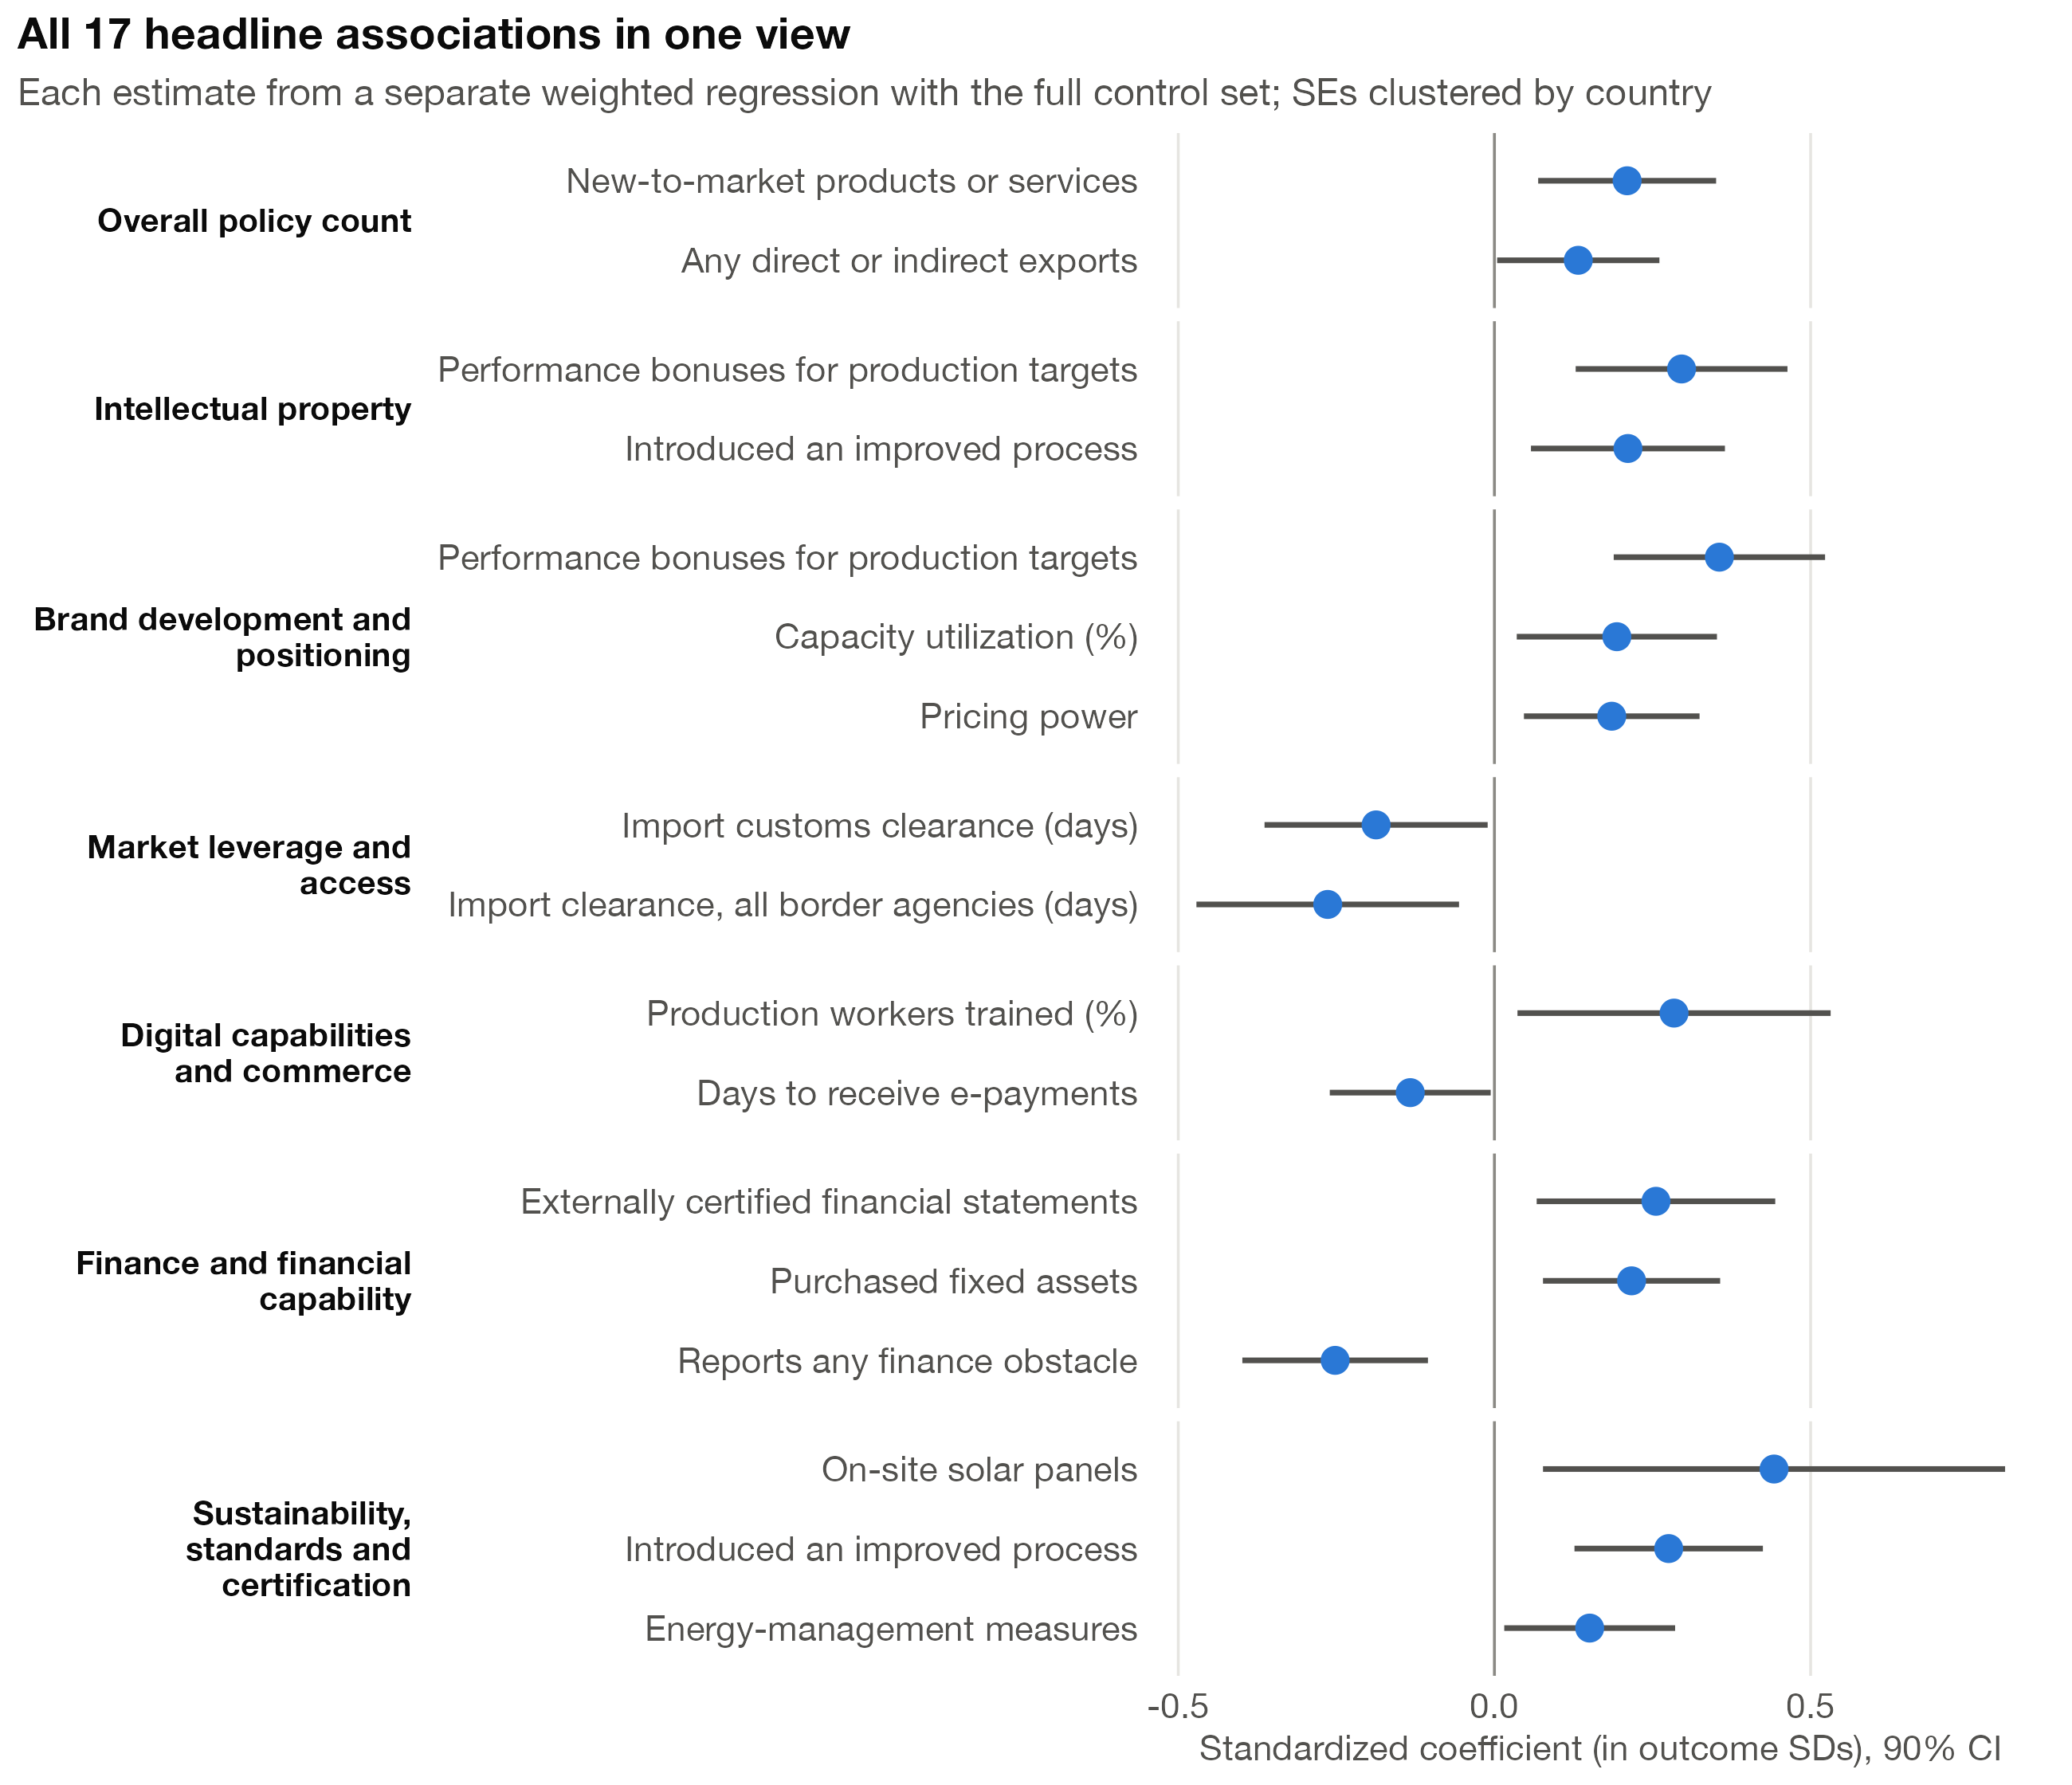
\includegraphics[width=0.92\linewidth]{figA1_all_coefficients.png}
  \figsource{Note: Points are coefficients divided by the weighted outcome standard deviation; bars are 90\% confidence intervals from country-clustered standard errors.}
\end{figure}

\begin{table}[H]
  \caption{Adjusted differences between high- and low-exposure country-waves}\label{tab:reg}
  \small
  \resizebox{\linewidth}{!}{\begin{tabular}{@{}l r r c r r r@{}}
\toprule
Outcome & Estimate & Std.\ error & 90\% CI & $p$ & Firms & Countries \\
\midrule
\multicolumn{7}{@{}l}{\textbf{Overall policy count}} \\
\quad Any direct or indirect exports & $+$6.4 pp$^{*}$ & 3.7 & [0.2, 12.5] & 0.094 & 10,356 & 72 \\
\quad New-to-market products or services & $+$10.0 pp$^{**}$ & 4.1 & [3.3, 16.6] & 0.017 & 2,540 & 70 \\
\addlinespace
\multicolumn{7}{@{}l}{\textbf{Intellectual property}} \\
\quad Introduced an improved process & $+$9.6 pp$^{**}$ & 4.2 & [2.6, 16.6] & 0.027 & 10,426 & 72 \\
\quad Performance bonuses for production targets & $+$14.8 pp$^{***}$ & 5.1 & [6.4, 23.2] & 0.005 & 7,246 & 72 \\
\addlinespace
\multicolumn{7}{@{}l}{\textbf{Brand development and positioning}} \\
\quad Pricing power & $+$8.5 pp$^{**}$ & 3.9 & [2.1, 14.9] & 0.031 & 6,490 & 67 \\
\quad Capacity utilization (\%) & $+$4.2 pp$^{**}$ & 2.1 & [0.8, 7.6] & 0.048 & 8,579 & 71 \\
\quad Performance bonuses for production targets & $+$17.8 pp$^{***}$ & 5.1 & [9.4, 26.1] & $<$0.001 & 7,246 & 72 \\
\addlinespace
\multicolumn{7}{@{}l}{\textbf{Market leverage and access}} \\
\quad Import customs clearance (days) & $-$2.6 days$^{*}$ & 1.5 & [$-$5.1, $-$0.2] & 0.086 & 1,272 & 66 \\
\quad Import clearance, all border agencies (days) & $-$6.4 days$^{**}$ & 3.1 & [$-$11.5, $-$1.4] & 0.042 & 793 & 46 \\
\addlinespace
\multicolumn{7}{@{}l}{\textbf{Digital capabilities and commerce}} \\
\quad Days to receive e-payments & $-$0.9 days$^{*}$ & 0.5 & [$-$1.8, $-$0.04] & 0.090 & 6,379 & 67 \\
\quad Production workers trained (\%) & $+$10.4 pp$^{*}$ & 5.5 & [1.3, 19.5] & 0.063 & 2,391 & 69 \\
\addlinespace
\multicolumn{7}{@{}l}{\textbf{Finance and financial capability}} \\
\quad Reports any finance obstacle & $-$12.3 pp$^{***}$ & 4.4 & [$-$19.5, $-$5.2] & 0.006 & 10,326 & 72 \\
\quad Externally certified financial statements & $+$12.8 pp$^{**}$ & 5.7 & [3.3, 22.2] & 0.029 & 10,359 & 72 \\
\quad Purchased fixed assets & $+$10.8 pp$^{**}$ & 4.2 & [3.8, 17.7] & 0.013 & 10,403 & 72 \\
\addlinespace
\multicolumn{7}{@{}l}{\textbf{Sustainability, standards and certification}} \\
\quad On-site solar panels & $+$15.2 pp$^{*}$ & 7.6 & [2.6, 27.7] & 0.061 & 1,421 & 20 \\
\quad Energy-management measures & $+$7.4 pp$^{*}$ & 4.0 & [0.8, 14.0] & 0.071 & 7,159 & 69 \\
\quad Introduced an improved process & $+$12.5 pp$^{***}$ & 4.1 & [5.8, 19.3] & 0.003 & 10,426 & 72 \\
\bottomrule
\end{tabular}
}
  \figsource{Note: Each row is a separate regression with the full control set and fixed effects. ``pp'' = percentage points. 90\% CI = estimate $\pm$ 1.645 $\times$ country-clustered standard error. $^{*}p<0.10$, $^{**}p<0.05$, $^{***}p<0.01$.}
\end{table}

\section{Discussion}\label{sec:disc}

The patterns are consistent: in most channels, creative firms in countries whose policies focus more on that channel do better on related outcomes, and most differences hold after controls. Three limits matter for how the evidence is used.

\textbf{Associations, not effects.} Exposure varies only between countries, so other national differences may drive part of each gap, even after controls for income, population and infrastructure.

\textbf{Selected outcomes.} For each channel, the outcomes reported were chosen from a broader screen of WBES indicators as the most informative for that channel. With many outcomes screened, some differences will appear by chance, so the results describe where the patterns are and should be tested further before being treated as confirmed findings.

\textbf{Coverage.} UNESCO records depend on countries' reporting capacity. The WBES covers formal firms with five or more employees, so micro-enterprises, informal businesses and individual creators, a large part of the creative economy, are not observed. Channel scores measure how closely policy texts align with written definitions, not policy budgets, implementation or reach.

These limits also point to what would improve measurement of the creative economy: firm data that reach smaller and informal creative businesses, policy records with comparable coverage across income groups, and policy descriptions that state budgets and beneficiaries.

\section{Conclusion}

Policy focus can be measured from public text at scale, it differs meaningfully across countries, and it lines up with the outcomes creative firms report. The pipeline is open and reproducible: it can be rerun as new UNESCO reports and survey waves become available, extended to other text sources such as national IP strategies or copyright legislation, and used to monitor where policy attention for creative industries is concentrated and where it is missing.

\appendix
\renewcommand{\thetable}{A\arabic{table}}
\setcounter{table}{0}

\section{Variables and reproduction}\label{app:vars}

\begin{table}[H]
  \caption{Outcome definitions}\label{tab:vars}
  \small
  \begin{tabular}{@{}l l l@{}}
\toprule
Outcome (as labelled in figures) & WBES item & Unit in tables \\
\midrule
Pricing power & \texttt{e33} & share of firms; differences in pp \\
Capacity utilization (\%) & \texttt{f1} & percent; differences in pp \\
Performance bonuses for production targets & \texttt{r8} & share of firms; differences in pp \\
Days to receive e-payments & \texttt{k35} & days \\
Production workers trained (\%) & \texttt{l11a} & percent; differences in pp \\
Reports any finance obstacle & \texttt{k30} & share of firms; differences in pp \\
Externally certified financial statements & \texttt{k21} & share of firms; differences in pp \\
Purchased fixed assets & \texttt{k4} & share of firms; differences in pp \\
Introduced an improved process & \texttt{h5} & share of firms; differences in pp \\
Import customs clearance (days) & \texttt{d14a} & days \\
Import clearance, all border agencies (days) & \texttt{d40a} & days \\
Any direct or indirect exports & \texttt{d3b, d3c} & share of firms; differences in pp \\
New-to-market products or services & \texttt{h2} & share of firms; differences in pp \\
On-site solar panels & \texttt{c43} & share of firms; differences in pp \\
Energy-management measures & \texttt{ge8d} & share of firms; differences in pp \\
\bottomrule
\end{tabular}

  \figsource{Note: WBES item codes refer to the Enterprise Surveys comprehensive file. ``Any direct or indirect exports'' is constructed from the direct and indirect export shares of sales (\texttt{d3b}, \texttt{d3c}); ``Reports any finance obstacle'' equals 1 if access to finance (\texttt{k30}) is rated as any obstacle.}
\end{table}

The full pipeline is public: the Python scorer for the policy texts, the Stata do-file for the sample, descriptive statistics and regressions, and R scripts that generate every figure and table in this paper from the saved results. The WBES microdata, the UNESCO records and the World Development Indicators are downloaded from their public portals.

\section{Channel definitions}\label{app:channels}

The six channels are the focus areas of Chapter~4 of the \emph{SME Competitiveness Outlook 2027}. For each channel, the text below (its name, role, definition, signal terms and exclusions) is combined into one passage and embedded with the same model as the policy records; each record's score for the channel is its similarity to that passage. The definitions are also in the repository as \texttt{smeco2027\_six\_channel\_definitions.csv}.

{\small
\subsection*{B.1\quad Intellectual property}
\emph{Core value-capture transition: from creators of content to owners of IP.}

Policies, programmes, laws, institutions or practical services that help creative SMEs identify, document, protect, retain, exploit and manage intangible creative assets so they can earn income beyond a one-off sale. This includes copyright, related rights, trademarks, design rights, patents, geographical indications, trade secrets, contracts, chain of title, licensing, royalties, collective management, anti-piracy, enforcement, rights metadata and IP-backed or royalty-based monetisation.

\textbf{Terms that signal the channel:} copyright; intellectual property; authors' rights; related rights; neighbouring rights; trademark; design right; patent; geographical indication; trade secret; licensing; royalties; royalty collection; collective management organization; CMO; anti-piracy; enforcement; rights retention; contract; chain of title; ownership; intangible asset; IP-backed lending; rights metadata; registry; creator compensation; fair remuneration.

\textbf{Excluded or down-weighted:} generic cultural heritage, creativity, innovation or entrepreneurship language without ownership, protection, licensing, royalties, contracts or monetisation of intangible assets.

\subsection*{B.2\quad Brand development and positioning}
\emph{Core value-capture transition: from suppliers to builders of brands.}

Policies or services that help creative SMEs convert distinctiveness, origin, quality, identity and reputation into market recognition, price premia, repeat demand and direct audience or customer relationships. This includes brand strategy, positioning, packaging, storytelling, marketing, social media presence, owned channels, trademarks when used for brand identity, reputation-building, buyer recognition, diaspora/audience development and visible crediting of creators or firms.

\textbf{Terms that signal the channel:} brand; branding; brand identity; positioning; market recognition; reputation; origin story; storytelling; packaging; label; logo; trademark for brand identity; price premium; willingness to pay; repeat demand; customer loyalty; audience relationship; owned channel; mailing list; social media presence; visible credit; promotion; influencer; diaspora marketing; cultural distinctiveness.

\textbf{Excluded or down-weighted:} generic SME support, start-up support, incubators, productivity or scaling language without recognition, positioning, reputation, customer relationship or price-premium logic.

\subsection*{B.3\quad Market leverage and access}
\emph{Core value-capture transition: from intermediary dependence to market leverage.}

Policies, infrastructure or services that help creative SMEs reach buyers and audiences on better terms, diversify routes to market, reduce dependence on gatekeepers and intermediaries, negotiate deliberately, control customer access or data, and build bargaining power individually or collectively. This includes export promotion, showcases, fairs, mobility, distribution, e-commerce routes, direct-to-consumer sales, platform access, buyer linkages, logistics, customs, certification for market entry and collective bargaining or producer organizations.

\textbf{Terms that signal the channel:} market access; export promotion; distribution; route to market; buyer linkage; audience access; fair; showcase; festival; mobility; touring; residency; direct-to-consumer; direct-to-fan; platform access; marketplace; intermediary; gatekeeper; bargaining; negotiation; collective bargaining; producer organization; cooperative; customer data; first-party data; distributor; sales agent; customs; logistics; parcel shipment; market intelligence.

\textbf{Excluded or down-weighted:} generic trade openness or infrastructure language that does not affect creative SMEs' access to buyers, audiences, distribution channels or negotiating position.

\subsection*{B.4\quad Digital capabilities and commerce}
\emph{Enabling condition: digital tools that make ownership, branding and market leverage cheaper or more feasible.}

Policies or programmes that improve creative SMEs' capacity to use digital tools for creation, rights management, audience-building, commerce, analytics and distribution. The definition should privilege firm-facing digital adoption that helps SMEs own assets, build brands, reach customers, collect revenues, monitor use and reduce intermediary dependence.

\textbf{Terms that signal the channel:} digital tool; digital transformation; e-commerce; online sales; platform; website; social media; newsletter; community platform; streaming; direct-to-fan; digital rights management; DRM; content ID; online registry; metadata; licensing marketplace; royalty tracking; usage monitoring; analytics; first-party data; search engine optimization; online marketing; AI translation; subtitling; dubbing; digital payment; broadband; internet.

\textbf{Excluded or down-weighted:} generic government digitalization, statistics systems or public-sector ICT modernization without a firm-facing link to creative production, IP, branding, commerce, payments, distribution or analytics.

\subsection*{B.5\quad Finance and financial capability}
\emph{Enabling condition: the right money at the right stage for intangible-rich creative SMEs.}

Policies, funds, instruments or advisory services that help creative SMEs finance the creation, protection, monetisation and scaling of intangible assets without losing ownership or strategic control. This includes grants for rights registration, concessional finance, working capital, invoice factoring, trade finance, export credit, credit guarantees, crowdfunding, royalty/revenue-based finance, IP-backed lending, investment readiness, business planning, financial records and separating business from personal accounts.

\textbf{Terms that signal the channel:} access to finance; grant; concessional finance; loan; credit; line of credit; guarantee; equity; investment readiness; business plan; financial records; working capital; invoice factoring; receivables; trade finance; export credit; credit insurance; crowdfunding; revenue-based finance; royalty financing; IP-backed lending; collateral; cash flow; payment delay; bank account; savings account; financial management.

\textbf{Excluded or down-weighted:} generic public spending, subsidies or macro-finance language that does not improve creative SMEs' access to capital, cash-flow management, investment readiness or intangible-asset monetisation.

\subsection*{B.6\quad Sustainability, standards and certification}
\emph{Enabling condition: sustainability as credible differentiation and market access, not only compliance.}

Policies, standards, certifications or services that help creative SMEs adopt verifiable environmental, social, quality or safety practices, including eco-labelling, traceability, sustainable materials, circular production, energy management, clean energy, audits, certification, compliance systems and buyer-trust standards. The emphasis is on concrete firm practices and credible standards, not broad sustainable-development rhetoric.

\textbf{Terms that signal the channel:} sustainability; environmental practice; social standard; certification; quality certification; eco-label; traceability; responsible sourcing; circular design; circular economy; sustainable materials; waste management; recycling; carbon; emissions; energy management; clean energy; solar; green production; compliance; due diligence; audit; inspection; product passport; fair trade; buyer trust; anti-greenwashing.

\textbf{Excluded or down-weighted:} generic sustainable development, cultural diversity, social inclusion or environmental rhetoric without concrete firm practices, energy management, clean energy, standards, certification, compliance, traceability, audits or buyer credibility.


}

\end{document}
